\documentclass[a4paper,11pt]{report}

\usepackage[utf8]{inputenc}
\usepackage[only,llbracket,rrbracket]{stmaryrd}
\usepackage{a4wide}
\usepackage[a4paper]{geometry}
\usepackage{mathtools}
\usepackage[T1]{fontenc}
\usepackage{lmodern}
\usepackage{hyperref}
\usepackage{subcaption}
\usepackage{placeins}
\usepackage{amssymb}
\usepackage{fixltx2e}
\usepackage{natbib}
\usepackage[crop=pdfcrop,process=auto]{pstool}
\usepackage{multirow}
\usepackage{enumerate}
%\usepackage[notref]{showkeys}
\usepackage{todonotes}

%\renewcommand*\showkeyslabelformat[1]{\normalfont\tiny#1}

\numberwithin{equation}{section}

\newcommand{\Sst}[1]{^\text{\tiny #1}}
\newcommand{\sst}[1]{_\text{\tiny #1}}

\newcommand{\diff}[2]{\frac{\mathrm{d} #1}{\mathrm{d} #2}}
\newcommand{\pdiff}[2]{\frac{\partial #1}{\partial #2}}
\newcommand{\V}[1]{\mathbf{#1}}
\newcommand{\E}[1]{\langle #1 \rangle}
\newcommand{\Pe}{\mathrm{Pe}}
\newcommand{\Da}{\mathrm{Da}}
\newcommand{\dd}[1]{\,\mathrm{d} #1}
\newcommand{\jump}[1]{\left\llbracket #1 \right\rrbracket}
\newcommand{\bo}[1]{O(#1)}
\newcommand{\lo}[1]{o(#1)}
\newcommand{\ti}[1]{\widetilde{#1}}

\bibliographystyle{plainnat}

\title{Transport processes in spatially disordered media}
\author{Matthew Russell}
\date{\today}

\begin{document}
\maketitle

\tableofcontents

\chapter{Introduction}
The problem of the transport of a solute arises in many areas of science. In
physiology, examples include the transport of nutrients from the maternal to the
foetal blood in the placenta (see figure~\ref{fig:placenta}; the exchange of oxygen
and carbon dioxide by the alvioli in the lungs (see figure~\ref{fig:alveolus}).

\begin{figure}[ht!]
    \centering
    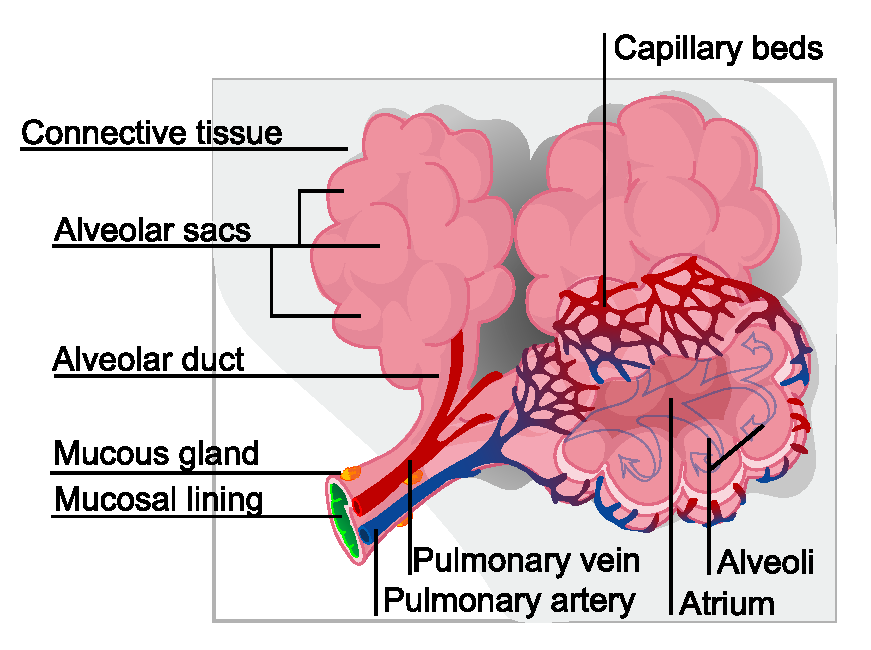
\includegraphics[width=0.7\textwidth]{introduction/figures/alveolus}
    \caption{\label{fig:alveolus}Schematic of an alveolar acini (from
http://en.wikipedia.org/wiki/File:Alveolus\_diagram.svg)}
\end{figure}
\begin{figure}[ht!]
    \centering
    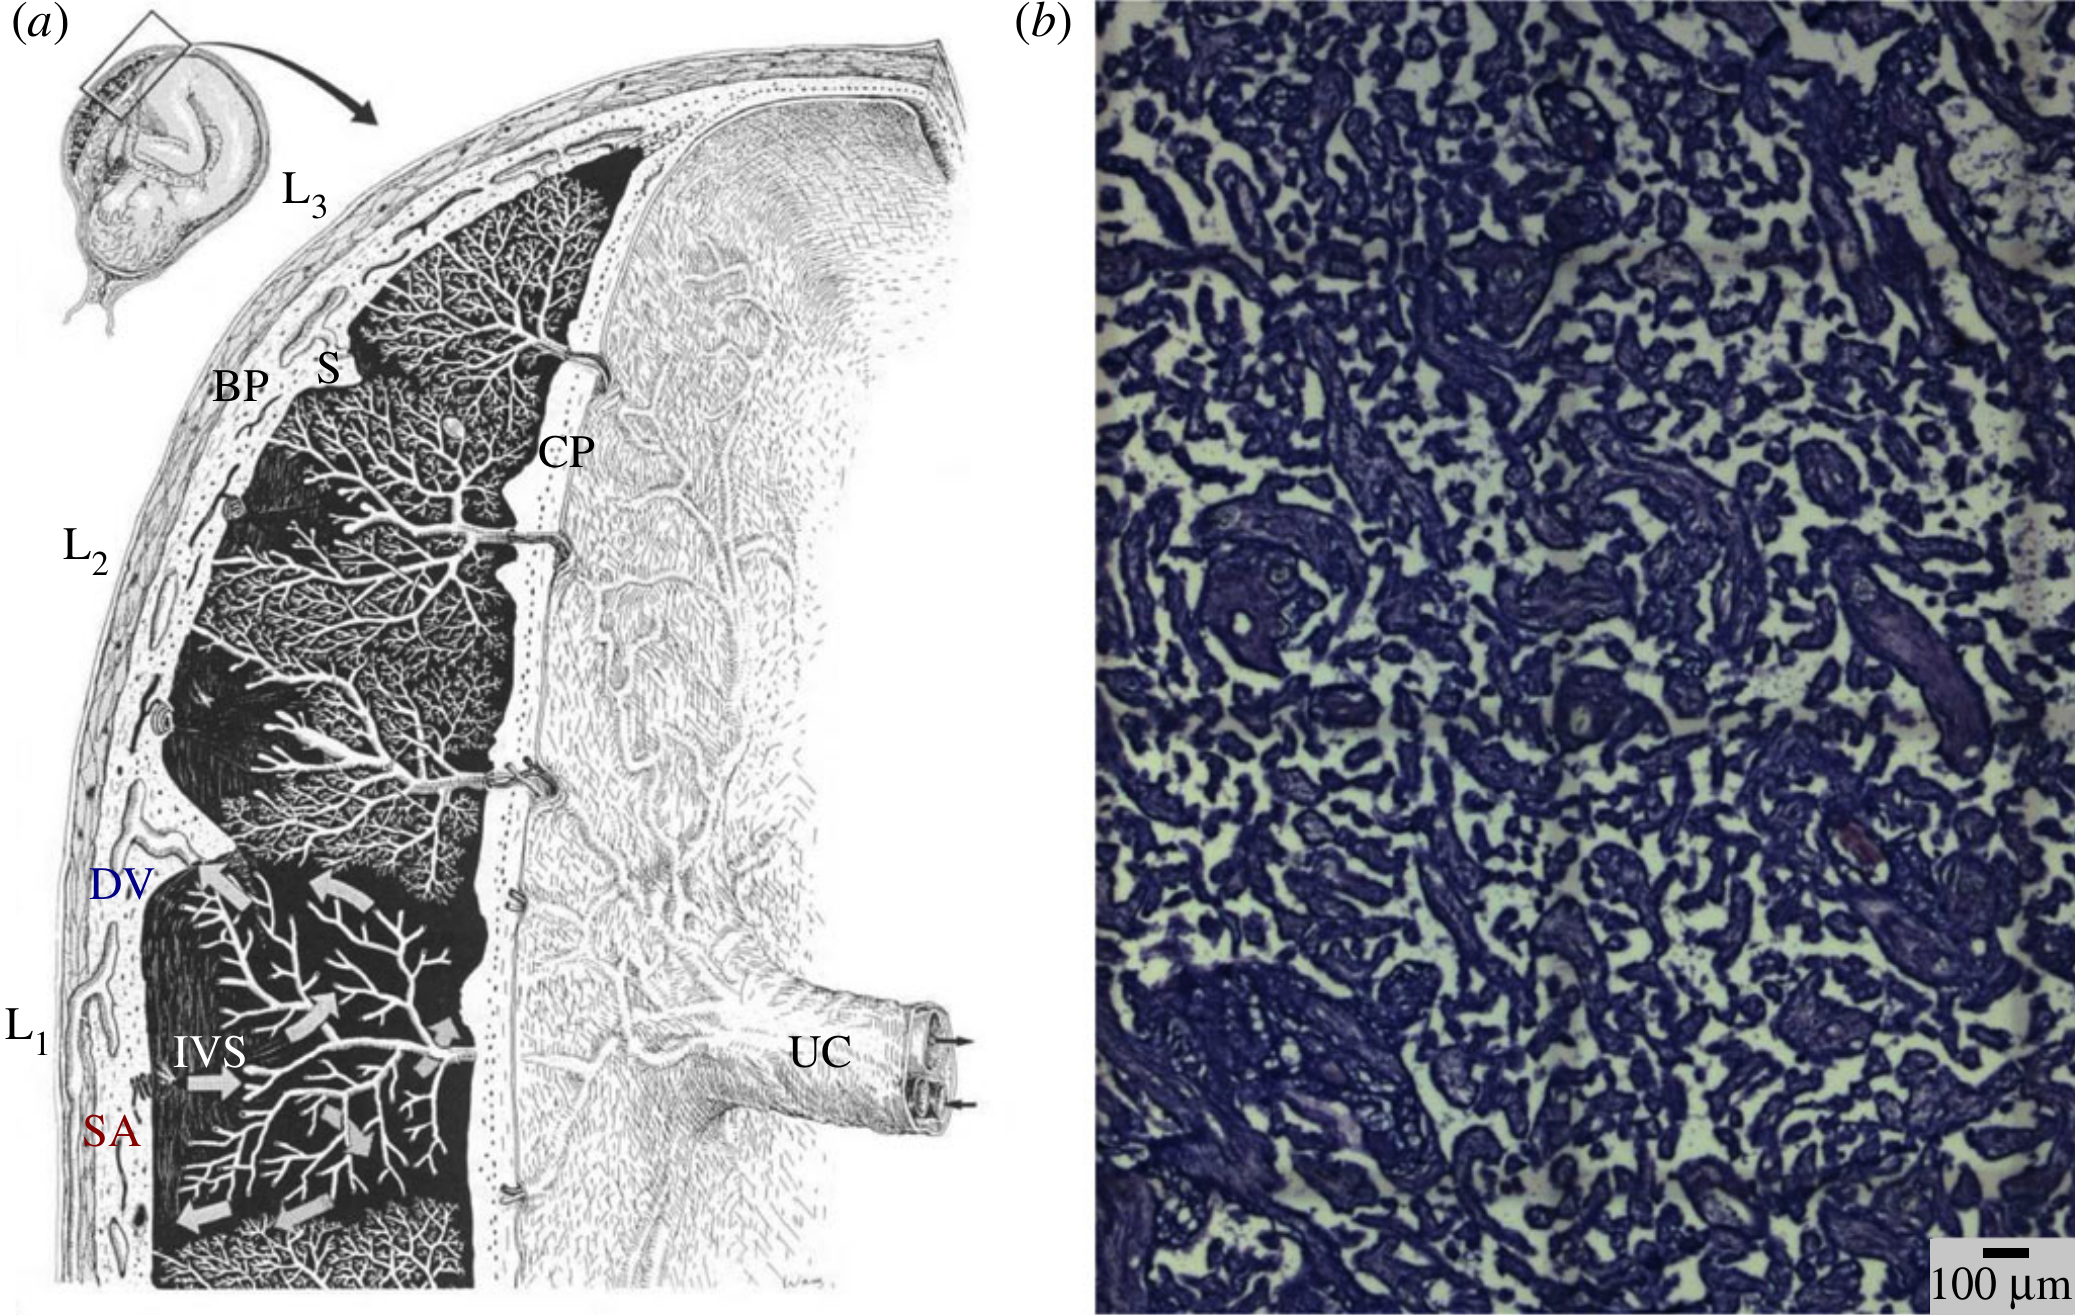
\includegraphics[width=0.7\textwidth]{introduction/figures/placentarast}
    \caption{\label{fig:placenta}Schematic of the placenta (from
    \cite{chernyavsky2012characterizing})}
\end{figure}

\todo{More examples? Other fields - earth science, industry \ldots}

We use two broad approaches to model transport phenomena: continuum models and
agent based models. The relationship between these approaches is another focus
and a goal is to provide a unified model incorporating features of both types of
model.

Both approaches assign a representation of concentration to each
spatial location. In continuum models, physical space is represented as an
interval of the real numbers and the concentration takes positive real values.
In contrast, the most basic individual based models involve finitely many
spatial locations (called ``urns'') and each urn can hold a positive integral
number of particles.

When one begins to take certain limits of the individual based system, the
distinction between the two approaches becomes less well-defined. For example,
one may obtain a continuum model from a discrete model in the appropriate limits
of a large number of urns and large numbers of particles. \todo{clarify, refs}

\section{Literature review}
\subsection{Transport phenomena in physiology and biology}
Transport phenomena are ubiquitous in physiological and biological systems and
can been seen on a vast range of time- and length-scales.

\begin{itemize}
    \item placenta
    \item lung \cite{grebenkov2005diffusion}
    \item ion channels
    \item ants (traffic)
\end{itemize}

\subsection{Individual based models}
\todo{\cite{schadschneider2010stochastic} reserve ``individual'' for
non-stochastic models, and ``population'' stochastic}

An individual based approach models a transport problem by analysing the
stochastic interactions between discrete entities in a population.
\citet{van2007stochastic} and \citet{gardiner2009stochastic} give thorough
accounts of general stochastic processes. Generally, physical space is
discretised into a finite set of locations, which we will refer to as ``urns'',
which each hold a number of particles. Different types of models are based on
the capacity of the urns and whether time is represented as a discrete or
continuous variable. For example, exclusion processes (REF) and zero range
processes REF blah.

%Applying this approach to the problem of solute transport, the entities
%represent the particles of the solute. The physical interaction of the particles
%with each other gives rise to macroscopic phenomena such as diffusion. The
%particle-scale interactions are modelled by a set of \emph{events}, which are
%problem specific. Once the microscopic properties of an individual based model
%have been specified, it is possible to create realisations of the system using a
%stochastic simulation algorithm --- for example, the Gillespie algorithm
%(described below). The model is random in nature, with the events being randomly
%selected from an appropriate probability distribution. As such, in order to find
%the statistical properties of the system, an ensemble of realisations can be
%created from which properties can be estimated. In addition to this, we can make
%theoretical predictions (in some cases, exact expressions, and in others,
%approximations) of the statistical properties of an individual based system.
%These are typically derived from a Master equation, which describes the time
%evolution of the probability distribution defining the system.

The two main types of randomness in individual based models are
\begin{itemize}
    \item Intrinsic noise --- randomness arising from the stochastic nature of the
        physical problem;
    \item Quenched disorder --- randomness of a parameter of the system which is
        usually chosen and fixed before allowing the system to evolve.
\end{itemize}
In solute transport in a disordered medium, a source of quenched disorder is the
randomness of the sink locations.
\todo{elaborate?}

We are interested in macroscopic features of the system, including their
statistics, which are expected to arise from both types of disorder and their
interactions.

\begin{itemize}
    \item General stochastic processes \cite{van2007stochastic},
        \cite{gardiner2009stochastic}
    \item General stochastic processes and specifically transport processes
        \cite{schadschneider2010stochastic}
    \item Exclusion processes
    \item Zero range processes (apparently introduced in
        \cite{spitzer1970interaction})
        \begin{itemize}
            \item There is a mapping from exclusion processes to ZRPs (under
                certain conditions)
            \item ZRPs exhibit a ``condensation transition analogous to
                Bose-Einstein condensation''
            \item It's ``known'' that ZRPs in a 1D periodic domain have a
                factorisable pdf in steady state (Schadscheider et al)
            \item Their exact steady state solution is also ``known''
                (Schadscheider et al)
            \item ``Zero-range process with open boundaries'' gives the
                open-boundaries stationary distribution (our problem)
        \end{itemize}
    \item ``Quantum formalism'' of the master equation allows analogies
        with quantum spin chains to be made
\end{itemize}

\subsubsection{Stochastic simluation}
\begin{itemize}
    \item Gillespie \cite{gillespie1976general} \cite{gillespie1977exact}
    \item Others (next reaction method etc.) \cite{anderson2007modified} gives
        summary of a few
    \item These give single realisations --- obtain estimates of distributions
        of observables from Monte-Carlo
    \item Cheap to run
    \item Useful when closed-form expressions for distributions are difficult or
        impossible to find
\end{itemize}

\subsection{Continuum based models}
\cite{chernyavsky2011transport} \cite{chernyavsky2012characterizing}
others\ldots


\chapter{Individual based approach}
\section{Problem formulation}
In one dimension, we formulate the problem by discretising space into a
finite set of locations at equal intervals. To each spatial location (``urn'') we assign
a non-zero number of particles and particles can move from one urn to
another according to the set of events.

\begin{figure}[ht!]
    \centering
    \psfragfig[width=0.6\textwidth]{individual/figures/urns}
    {
        \psfrag{1}{\(1\)}
        \psfrag{2}{\(2\)}
        \psfrag{3}{\(3\)}
        \psfrag{N-1}{\(N-1\)}
        \psfrag{N}{\(N\)}
    }
    \caption{\label{fig:urns}Set up of the urns containing the particles}
\end{figure}

The different types of events in our problem are as follows:
\begin{table}[ht!]
    \centering
    \begin{tabular}{ c | c | c }
        Description & Effect & Count \\ \hline\hline
        \multirow{2}{*}{Hop left} & \(n_{i+1} \leftarrow n_{i+1} - 1\) & \multirow{2}{*}{\(N-1\)} \\ & \(n_i \leftarrow n_i + 1\) \\ \hline
        \multirow{2}{*}{Hop right} & \(n_i \leftarrow n_i - 1\) & \multirow{2}{*}{\(N-1\)} \\ & \(n_{i+1} \leftarrow n_{i+1} + 1\) \\ \hline
        Inflow & \(n_1 \leftarrow n_1 + 1\) & \(1\) \\ \hline
        Outflow & \(n_N \leftarrow n_N - 1\) & \(1\) \\ \hline
        Removal & \(n_i \leftarrow n_i - 1\) & \(N\) \\
    \end{tabular}
    \caption{\label{tab:generic_transport_events}Definitions of the different types of
events in the solute transport system}
\end{table}

Figure~\ref{fig:transport_events} gives a diagrammatic representation of the
different event types in terms of the urns.

\begin{figure}[ht!]
    \centering
    \begin{subfigure}[b]{0.3\textwidth}
        \centering
        \psfragfig{individual/figures/hopleft}
        {
            \psfrag{i}{\(i\)}
            \psfrag{i+1}{\(i+1\)}
        }
        \caption{Hop left}
    \end{subfigure}
    \qquad\qquad
    \begin{subfigure}[b]{0.3\textwidth}
        \centering
        \psfragfig{individual/figures/hopright}
        {
            \psfrag{i}{\(i\)}
            \psfrag{i+1}{\(i+1\)}
        }
        \caption{Hop right}
    \end{subfigure}

    \begin{subfigure}[b]{0.3\textwidth}
        \centering
        \psfragfig{individual/figures/inflow}
        {
            \psfrag{1}{\(1\)}
        }
        \caption{Inflow}
    \end{subfigure}
    \qquad\qquad
    \begin{subfigure}[b]{0.3\textwidth}
        \centering
        \psfragfig{individual/figures/outflow}
        {
            \psfrag{N}{\(N\)}
        }
        \caption{Outflow}
    \end{subfigure}

    \begin{subfigure}[b]{0.3\textwidth}
        \centering
        \psfragfig{individual/figures/removal}
        {
            \psfrag{i}{\(i\)}
        }
        \caption{Removal}
    \end{subfigure}
    \caption{\label{fig:transport_events}Diagrammatic representation of the
different event types in the solute transport system}
\end{figure}

\section{Gillespie algorithm}
The Gillespie algorithm is a stochastic simulation algorithm, named after
Gillespie due to the papers \cite{gillespie1976general,gillespie1977exact}. It
was described by Gillespie in terms of its application to simulating chemical
reactions, but it is applicable to any continuous time Markov process.
\cite{anderson2007modified} gives a clear description of the algorithm (again in
terms of chemical reactions).

Suppose we have a physical system with \(N\) possible ``urns'' that each
particle can reside in (we impose no upper limit on the number of particles in
each urn), as in figure~\ref{fig:urns}. The urns could correspond to physical
locations or chemical species, for example. Denote the number of particles in
urn \(i\) by \(n_i\). Also suppose that there are \(M\) different events that
can occur in the system, such as a particle moving from one urn to the adjacent
urn (as in physically moving in space or a chemical reaction), or the
spontaneous appearance of a particle in the first urn. These events must occur
at specified rates, which represent the number of times per second one expects
the corresponding event to occur.  Given the rates \(T_i, 1 \le i \le M\) at
which the events in the system are expected to occur, the basic idea of the
Gillespie algorithm is to randomly choose the time increment and then randomly
choose the event that will occur at the new time. The random time increment is
drawn from an exponential distribution with parameter \(T_0 = \sum_{i=1}^M
T_i\), the sum of all of the rates. The rates of the events are not necessarily
constants and therefore must be recalculated at each time step. For example, the
rate at which a particle jumps from one urn to an adjacent urn might depend on
the number of particles in the original urn.

The Gillespie algorithm is as follows:
\begin{enumerate}[\bfseries Step 1:]
    \item Set the initial number of particles in each urn and set time \(t=0\)
    \item Calculate the rate \(T_i\) for each of the \(M\) events
    \item Set \(T_0 = \sum_{i=1}^M T_i\)
    \item Generate a uniformly random real number \(r\), such that \(0 \le r \le 1\)
    \item Set \(\delta t = \ln\left(\frac{1}{r}\right)/T_0\) (i.e. \(\delta t\)
        is drawn from an exponential distribution)
    \item Choose a event randomly from the discrete distribution such that
        probability of drawing event \(k\) is \(T_k/T_0\), for \(1 \le k \le
        M\)
    \item Increment time according to the time step, \(t \leftarrow t + \delta
        t\), and perform the changes corresponding to the event chosen
    \item Return to Step 2, unless the stopping criteria have been met
\end{enumerate}

\section{Zeroth order solute transport}
Zeroth order transport implies that the rates of removal and outflow of
particles do not depend on the number of particles. In other words, the rates
are constants. This can causes the unphysical problem of negative particle numbers if the
rates are high enough. Clearly, when an urn is empty, no particles can be
removed from it. Therefore, we multiply the removal rates by the discrete
Heaviside function,
\begin{equation*}
    H(n) =
    \begin{dcases*}
        1 & if \(n \ge 1\)\\
        0 & if \(n < 1\)
    \end{dcases*}
\end{equation*}
 to ensure that the rates go to zero once the particle number reaches zero.

We can now augment the table~\ref{tab:generic_transport_events} to give the
rates assuming zeroth order removal kinetics:
\begin{table}[ht!]
    \centering
    \begin{tabular}{ c | c | c | c }
        Description & Rate & Effect & Count \\ \hline\hline
        \multirow{2}{*}{Hop left} & \multirow{2}{*}{\(T^-_i = a n_{i+1}\)} &
        \(n_{i+1} \leftarrow n_{i+1} - 1\) & \multirow{2}{*}{\(N-1\)} \\
        & & \(n_i \leftarrow n_i + 1\) \\ \hline
        \multirow{2}{*}{Hop right} & \multirow{2}{*}{\(T^+_i = (a+b) n_i\)} &
        \(n_i \leftarrow n_i - 1\) & \multirow{2}{*}{\(N-1\)} \\
        & & \(n_{i+1} \leftarrow n_{i+1} + 1\) \\ \hline
        Inflow & \(T\Sst{in} = c\) & \(n_1 \leftarrow n_1 + 1\) & \(1\) \\ \hline
        Outflow & \(T\Sst{out} = d H(n_N)\) & \(n_N \leftarrow n_N - 1\) & \(1\) \\ \hline
        Removal & \(T\Sst{rem}_i = S_i H(n_i)\) & \(n_i \leftarrow n_i - 1\) & \(N\) \\
    \end{tabular}
    \caption{\label{tab:zeroth_order_transport_events}Rates of the different types of
events in the solute transport system with zeroth order kinetics}
\end{table}
The constants \(a,b,c,d\) and the \(S_i\) are parameters which must be
specified, corresponding to the rates of diffusion, advection, inflow, outflow
and removal (from urn \(i\)), respectively. (Maybe it only makes sense to have
\(d=a+b\)?).

There are \(M=2(N-1) + 2 + N = 3N\) events in total.
%Note that since
%the removal rate is a constant this corresponds to zero-order kinetics, where
%the removal rate does not depend on the number of particles in the urn.

\FloatBarrier

\subsection{Example realisations}

\begin{figure}[ht!]
    \centering
    \psfragfig{individual/figures/realisation1}
    {
        \psfrag{t}{\(t\)}
    }

    \caption{\label{fig:exreal1}Realisation of the time evolution of the number
of particles in each urn. \(N=10,a=1,b=0.5,c=1000,d=1.5,e=0\).}
\end{figure}

\begin{figure}[ht!]
    \centering
    \psfragfig{individual/figures/realisation2}
    {
        \psfrag{t}{\(t\)}
    }

    \caption{\label{fig:exreal2}Realisation of the time evolution of the number
of particles in each urn. \(N=10,a=2,b=0,c=1000,d=2,e=0\).}
\end{figure}

\FloatBarrier

\section{Master equation}
The master equation describes the time evolution of the probability distribution
on the states of a continuous time Markov processes.

%Its general form is
%
%\begin{equation}
%    \label{eqn:master_eqn_general}
%    \diff{P(i,t)}{t} = \sum_j A_{ij} P(j,t),
%\end{equation}
%where \(P(i,t)\) is the probability that the system is in state with label \(i\)
%at time \(t\), and \(A_{ij}\) is a matrix of rate coefficients.

In the case of solute transport, the states of the system consist of the number
of particles contained in each urn at a given time. It is convenient to use a
vector to collect this data:
\begin{equation}
    \label{eqn:state_vector}
    \V{n} = \left(n_1,n_2, \dotsc, n_N\right)^{T}.
\end{equation}
Also, let \(T(\V{n}|\V{n}')\) denote the rate of transition from state \(\V{n}'\)
to state \(\V{n}\). Then the master equation is \citep{mckane2012stochastic}
\begin{equation}
    \label{eqn:master_eqn_rates}
    \diff{P(\V{n},t)}{t} = \sum_{\V{n}' \neq \V{n}} \left[ T(\V{n}|\V{n}')
        P(\V{n}',t) - T(\V{n}'|\V{n}) P(\V{n},t) \right].
\end{equation}

Here, \(P(\V{n},t) = P(\V{n},t | \V{n}_0, t_0)\) is defined as the conditional probability of finding the
system in state \(\V{n}\) at time \(t\) given the initial condition that at time
\(t_0\), the system was in state \(\V{n}_0\).

We will later be interested in various moments of the probability distribution
of the random vector \(\V{n}\) defined by \(P(\V{n},t)\).

First, define the vectors \(\V{e}_i = (0,\dotsc,0,1,0,\dotsc,0)^T\) as the
vector with a \(1\) in the \(i\)-th entry and a \(0\) in all others. Then the
\emph{expectation} of \(\V{n}\) at time \(t\) is given by
\begin{equation}
    \E{\V{n}}(t) = \sum_{i=1}^N \E{n_i}(t) \V{e}_i
    \label{eqn:expectation_n}
\end{equation}
where \(\E{n_i}(t)\) is the expected value of the number of particles in urn
\(i\) at time \(t\) and is given by
\begin{equation}
    \begin{aligned}
        \E{n_i}(t) =& \sum_{j=0}^\infty j P(n_i = j,t)\\
        =& \sum_{j=0} j
        \sum_{\substack{\V{n} \text{ s.t.} \\ n_i=j}} P(\V{n},t)\\
        =& \sum_{j=0} j
        \sum_{n_1} \dotso \sum_{n_{i-1}} \sum_{n_{i+1}} \dotso \sum_{n_N} P(\V{n},t)\\
        =& \sum_{\V{n}} n_i P(\V{n},t),
    \end{aligned}
    \label{eqn:expecation_n_i}
\end{equation}
where \(P(n_i = j,t)\) denotes the marginal distribution of \(n_i\).  More
generally, the expectation of any scalar function of the random variables, say
\(f(\V{n})\) is defined by
\begin{equation}
    \E{f(\V{n})}(t) = \sum_{\V{n}} f(\V{n}) P(\V{n},t).
    \label{eqn:expectation_f(n)}
\end{equation}

The variance of \(n_i\) is given by
\begin{equation}
    \begin{aligned}
        \sigma_i(t) &= \E{(n_i - \E{n_i})^2}\\
        &= \E{n_i^2} - \E{n_i}^2,
    \end{aligned}
    \label{eqn:variance_n_i}
\end{equation}
and the covariance between \(n_i\) and \(n_j\) by
\begin{equation}
    \begin{aligned}
        \sigma_{ij}(t) &= \E{(n_i - \E{n_i})(n_j - \E{n_j})}\\
        &= \E{n_i n_j} - \E{n_i} \E{n_j}.
    \end{aligned}
    \label{eqn:covariance_n_i_n_j}
\end{equation}

\subsection{Jump moments}
In order to simplify the derivation of moments of the probability distribution
from the master equation, we can introduce the discrete multivariate jump
moments. To motivate their definition, we take the time derivative of the
expectation of the \(i\)-th random variable as follows. (Justification for
taking derivative inside infinite sum?)
\begin{align*}
    \diff{\E{n_i}}{t} &= \diff{}{t}\sum_{\V{n}}n_i P(\V{n},t)\\
    &= \sum_{\V{n}}n_i \diff{P(\V{n},t)}{t}\\
    &= \adjustlimits\sum_{\V{n}}\sum_{\V{n}'} n_i \left[ T(\V{n}|\V{n}') P(\V{n}',t) -
    T(\V{n}'|\V{n}) P(\V{n},t)\right]\\
    &= \adjustlimits\sum_{\V{n}}\sum_{\V{n}'} n_i T(\V{n}|\V{n}') P(\V{n}',t) -
    \adjustlimits\sum_{\V{n}}\sum_{\V{n}'} n_i T(\V{n}'|\V{n}) P(\V{n},t)\\
    &= \adjustlimits\sum_{\V{n}}\sum_{\V{n}'} n_i' T(\V{n}'|\V{n}) P(\V{n},t) -
    \adjustlimits\sum_{\V{n}}\sum_{\V{n}'} n_i T(\V{n}'|\V{n}) P(\V{n},t)\\
    &= \adjustlimits\sum_{\V{n}}\sum_{\V{n}'} (n_i' - n_i) T(\V{n}'|\V{n})
    P(\V{n},t),
\end{align*}
where we have substituted in the master equation \eqref{eqn:master_eqn_rates}.
This suggests that we define
\begin{equation}
    \begin{gathered}
        a_{\nu i}(\V{n}') = \sum_{\V{n}} (n_i'-n_i)^\nu T(\V{n}'|\V{n})\\
        (\nu = 0,1,2,\dotsc,\quad i=1,2,\dotsc)
    \end{gathered}
    \label{eqn:jump_moment}
\end{equation}
since then we have
\begin{equation}
    \diff{\E{n_i}}{t} = \E{a_{1i}(\V{n})},
    \label{eqn:time_evo_expectation_jump_moment}
\end{equation}
and we call \(a_{\nu i}(\V{n})\) the \emph{\(\nu\)-th jump moment of \(n_i\)}.

\subsubsection{Linear jump moments}
If we assume that we can write the \(\nu\)-th jump moment as a linear function of
\(\V{n}\), i.e. that
\begin{equation}
    a_{\nu i}(\V{n}) = \sum_{j=1}^{N} \alpha_{\nu i j} n_j + \beta_{\nu i},
    \label{eqn:linear_jump_moments_coeffs}
\end{equation}
for constants \(\alpha_{\nu i j}, \beta_{\nu i}\),
then, by linearity of the expectation, we have
\begin{equation}
    \E{a_{\nu i}(\V{n})} = a_{\nu i}(\E{\V{n}}).
    \label{eqn:linear_jump_moments}
\end{equation}

\subsubsection{Second moments}
We can perform the same trick for the second raw moment as we did for the
expectation, by which we obtain
\begin{equation}
    \begin{aligned}
        \diff{\E{n_i^2}}{t} &= \diff{}{t} \sum_{\V{n}} n_i^2 P(\V{n},t)\\
        &= \sum_{\V{n}} n_i^2 \diff{P(\V{n},t)}{t}\\
        &= \adjustlimits\sum_{\V{n}} \sum_{\V{n}'} ({n_i'}^2 - n_i^2) T(\V{n}' |
        \V{n}) P(\V{n},t)\\
        &= \adjustlimits\sum_{\V{n}} \sum_{\V{n}'} \left[ (n_i' - n_i)^2 + 2n_i(n_i'
        - n_i) \right] T(\V{n}' | \V{n}) P(\V{n},t)\\
        &= \E{a_{2i}(\V{n})} + 2 \E{n_i a_{1i}(\V{n})},
    \end{aligned}
    \label{eqn:time_evo_second_moment_jump_moment}
\end{equation}
which is an exact expression involving the first and second jump moments.

For the time evolution of the variance, \(\sigma_i^2 = \E{n_i^2} - \E{n_i}^2\),
we can combine the results in \eqref{eqn:time_evo_expectation_jump_moment} and
\eqref{eqn:time_evo_second_moment_jump_moment}:
\begin{equation}
    \begin{aligned}
        \diff{\sigma_i^2}{t} &= \diff{\E{n_i^2}}{t} - 2 \E{n_i}\diff{\E{n_i}}{t}\\
        &= \E{a_{2i}(\V{n})} + 2\left( \E{n_i a_{1i}(\V{n})} - \E{n_i}
        \E{a_{1i}(\V{n})} \right),
    \end{aligned}
    \label{eqn:time_evo_variance_jump_moment}
\end{equation}
which is again an exact expression.

In the case that the first and second jump moments are both linear, hence
satisfying \eqref{eqn:linear_jump_moments}, we can write
\begin{equation*}
    a_{1i}(\V{n}) = \sum_{j=1}^N \alpha_{1ij} n_j + \beta_{1i}, \quad
    a_{2i}(\V{n}) = \sum_{j=1}^N \alpha_{2ij} n_j + \beta_{2i}.
\end{equation*}
Substituting into \eqref{eqn:time_evo_variance_jump_moment} gives
\begin{equation}
    \begin{aligned}
        \diff{\sigma_i^2}{t} &= a_{2i}(\E{\V{n}}) + 2\left[ \E{n_i (\alpha_{1i1}n_1 +
            \dotsb + \alpha_{1iN}n_N + \beta_{1i})} \right.\\
            &\left. \quad - \E{n_i} \E{ \alpha_{1i1}n_1 +
        \dotsb + \alpha_{1iN}n_N + \beta_{1i}} \right]\\
        &= a_{2i}(\V{n}) + 2\left( \alpha_{1i1}\E{n_i n_1} + \dotsb +
        \alpha_{1iN}\E{n_i n_N}\right.\\
        &\quad \left. - \alpha_{1i1}\E{n_i}\E{n_1} - \dotsb -
        \alpha_{1iN}\E{n_i}\E{n_N} \right)\\
        &= a_{2i}(\V{n}) + 2 \sum_{j=1}^N \alpha_{1ij}(\E{n_i n_j} -
        \E{n_i}\E{n_j})\\
        &= a_{2i}(\V{n}) + 2 \sum_{j=1}^N \alpha_{1ij}\sigma(n_i,n_j),
    \end{aligned}
\end{equation}
where \(\sigma(n_i, n_j)\) is the covariance between \(n_i\) and \(n_j\).
This shows that, in general, when the process is such that the first two jump
moments are linear, the time evolution of the variance depends explicitly on the
covariance matrix of the multivariate state \(\V{n}\). In practice, we might
expect many of the coefficients \(\alpha_{1ij}, \alpha_{2ij}\) to be zero. For
example, for a jump process in which a particle can jump between only adjacent
urns, the matrix \(\alpha_1 = (\alpha_{1ij})\) would have a tridiagonal
structure.

\subsubsection{Covariance}
Generalising the equation for the variance, we can derive an equation for the
time evolution of the covariance between \(n_i\) and \(n_j\).
\begin{equation}
    \begin{aligned}
        \diff{\sigma_{ij}}{t}
        &= \diff{\E{n_i n_j}}{t} - \E{n_i}\diff{\E{n_j}}{t} -
        \E{n_j}\diff{\E{n_i}}{t}\\
        &= \adjustlimits\sum_{\V{n}} \sum_{\V{n}'}\left(n_i' n_j' - n_i
        n_j\right)T(\V{n}' | \V{n})P(\V{n},t)\\
        & \quad - \E{n_i}\E{a_{1j}(\V{n})} - \E{n_j}\E{a_{1i}(\V{n})}.
    \end{aligned}
    \label{eqn:time_evo_covar_sum}
\end{equation}
Notice that
\begin{align*}
    n_i' n_j' - n_i n_j = (n_i' - n_i)(n_j' - n_j) + n_i(n_j' - n_j) + n_j(n_i'
    - n_i).
\end{align*}
This then allows us to write \eqref{eqn:time_evo_covar_sum} as
\begin{equation}
    \begin{aligned}
        \diff{\sigma_{ij}}{t} = \E{a_{1 i j}(\V{n})} +
        \E{(n_i - \E{n_i})a_{1j}(\V{n})} + \E{(n_j - \E{n_j})a_{1i}(\V{n})},
    \end{aligned}
    \label{eqn:time_evo_covar_jump_moments}
\end{equation}
where we have used the mixed jump moment between \(n_i\) and \(n_j\) given by
\begin{equation}
    a_{\nu i j}(\V{n}) = \sum_{\V{n}'} (n_i' - n_i)^\nu (n_j' - n_j)^\nu
    T(\V{n}' | \V{n}).
    \label{eqn:mixed_jump_moment_i_j}
\end{equation}

When \(a_{1ij}(\V{n})\) is linear, we have \(\E{a_{1ij}(\V{n})} =
a_{1ij}(\E{\V{n}})\), and when \(a_{1j}(\V{n})\) is linear we have
\begin{equation*}
    \E{(n_i - \E{n_i})a_{1j}(\V{n})} = \sum_{k=1}^N \alpha_{1jk} \sigma_{ki},
\end{equation*}
and similarly for the third term by swapping \(i \leftrightarrow j\). Notice
that this sum is a matrix multiplication, and if we define
\begin{equation}
    m_{ij} = \sum_{k=1}^N \alpha_{1ik}\sigma_{kj},
\end{equation}
we can write the equations for the covariances in the form
\begin{equation}
    \begin{aligned}
        \diff{\sigma_{ij}}{t} = a_{1 i j}(\E{\V{n}}) + m_{ij} + m_{ji}.
    \end{aligned}
    \label{eqn:time_evo_covar_linear_jump_moments}
\end{equation}

\section{Zeroth order kinetics}
For the above problem of solute transport, the transition rates in
table~\ref{tab:zeroth_order_transport_events} can be combined into a single object using the
notation introduced in the previous section:
\begin{equation}
    \label{eqn:transition_rates_zeroth_order}
    T(\V{n}|\V{n}') =% \left\{
        \begin{dcases*}
            a n'_{i+1} & for \(\V{n} = \V{n}' + \V{e}_i - \V{e}_{i+1},
            i=1,\dotsc,N-1\)\\
            (a+b) n'_i & for \(\V{n} = \V{n}' - \V{e}_i + \V{e}_{i+1},
            i=1,\dotsc,N-1\)\\
            c & for \(\V{n} = \V{n}' + \V{e}_1\)\\
            d H(n'_N) & for \(\V{n} = \V{n}' - \V{e}_N\)\\
            S_i H(n'_i) & for \(\V{n} = \V{n}' - \V{e}_i, i=1,\dotsc,N\)\\
            0 & otherwise
        \end{dcases*}
        %\right.,
\end{equation}
where \(\V{e}_i = (0,\dotsc,0,1,0,\dotsc,0)^T\) is the vector with a \(1\) in
the \(i\)-th entry and a \(0\) in all others. Using this we can write \(\V{n} =
\sum_{i=0}^{N} n_i \V{e}_i\). We will calculate the terms on the right hand side
of the master equation \eqref{eqn:master_eqn_rates} corresponding to each type
of event separately.

\begin{itemize}
    \item Hop left (\(\V{n} = \V{n}' + \V{e}_i - \V{e}_{i+1}\)):
        \begin{equation}
            \label{eqn:trans_me_hl_term}
            \sum_{i=1}^{N-1} \left[a(n_{i+1}+1) P(\V{n} - \V{e}_i +
                \V{e}_{i+1},t) - a n_{i+1} P(\V{n},t) \right]
        \end{equation}
    \item Hop right (\(\V{n} = \V{n}' - \V{e}_i + \V{e}_{i+1}\)):
        \begin{equation}
            \label{eqn:trans_me_hr_term}
            \sum_{i=1}^{N-1} \left[(a+b)(n_i+1) P(\V{n} + \V{e}_i -
                \V{e}_{i+1},t) - (a+b)n_i P(\V{n},t) \right]
        \end{equation}
    \item Inflow (\(\V{n} = \V{n}' + \V{e}_1\)):
        \begin{equation}
            \label{eqn:trans_me_in_term}
            cP(\V{n} - \V{e}_1,t) - c P(\V{n},t)
        \end{equation}
    \item Outflow (\(\V{n} = \V{n}' - \V{e}_N\)):
        \begin{equation}
            \label{eqn:trans_me_out_term}
            d H(n_N + 1) P(\V{n} + \V{e}_N,t) - d H(n_N) P(\V{n},t)
        \end{equation}
    \item Removal (\(\V{n} = \V{n}' - \V{e}_i\)):
        \begin{equation}
            \label{eqn:trans_me_rem_term}
            \sum_{i=1}^N \left[ S_i H(n_i + 1) P(\V{n} + \V{e}_i,t) - S_i H(n_i) P(\V{n},t)
                \right]
        \end{equation}
\end{itemize}

Combining \eqref{eqn:trans_me_hl_term}--\eqref{eqn:trans_me_rem_term}, we
obtain the master equation for this system:
\begin{equation}
    \label{eqn:trans_me}
    \begin{split}
        \diff{P(\V{n},t)}{t} = &
            \sum_{i=1}^{N-1} \left[a(n_{i+1}+1) P(\V{n} - \V{e}_i +
                \V{e}_{i+1},t) - a n_{i+1} P(\V{n},t) \right]\\
            +&\sum_{i=1}^{N-1} \left[(a+b)(n_i+1) P(\V{n} + \V{e}_i -
                \V{e}_{i+1},t) - (a+b)n_i P(\V{n},t) \right]\\
            +&cP(\V{n} - \V{e}_1,t) - c P(\V{n},t)\\
            +&d H(n_N + 1) P(\V{n} + \V{e}_N,t) - d H(n_N) P(\V{n},t)\\
            +&\sum_{i=1}^N \left[ S_i H(n_i + 1) P(\V{n} + \V{e}_i,t) - S_i
                H(n_i) P(\V{n},t)
                \right].
    \end{split}
\end{equation}

\subsection{Jump moments}

\subsection{Mean}

\subsection{Covariances}

%\subsection{Deterministic mean-field equations}
%The objective of this section is to obtain an equation governing the time
%evolution of the expected value of the number of particles in each urn.
%
%The expected value of the entire state \(\V{n}\) at time \(t\) is
%\begin{equation*}
%    \E{\V{n}}(t) = \sum_{i=1}^N \langle n_i \rangle(t) \V{e}_i,
%\end{equation*}
%where \(\E{n_i}(t)\) is the expected value of the number of particles in urn
%\(i\) at time \(t\) and is given by
%\begin{align*}
%    \E{n_i}(t) =& \sum_{j=0}^\infty j P(n_i = j,t)\\
%    =& \sum_{j=0} j
%    \sum_{\substack{\V{n} \text{ s.t.} \\ n_i=j}} P(\V{n},t)\\
%    =& \sum_{j=0} j
%    \sum_{n_1} \dotso \sum_{n_{i-1}} \sum_{n_{i+1}} \dotso \sum_{n_N} P(\V{n},t)\\
%    =& \sum_{\V{n}} n_i P(\V{n},t),
%\end{align*}
%where \(P(n_i = j,t)\) denotes the marginal distribution of \(n_i\).
%
%Differentiating \(\E{n_i}\) with respect to time,
%\begin{align*}
%    \diff{(\E{n_i}(t))}{t} =& \sum_{\V{n}} n_i \diff{(P(\V{n},t))}{t}.
%\end{align*}
%
%Substituting the expression \eqref{eqn:trans_me} into the above,
%\begin{subequations}
%\begin{align}
%    \label{eqn:trans_expectation_hl_term}
%    \diff{(\E{n_i}(t))}{t}
%    = & \sum_\V{n} n_i \sum_{j=1}^{N-1}
%    \left[a(n_{j+1}+1) P(\V{n} - \V{e}_j + \V{e}_{j+1},t) -
%        an_{j+1} P(\V{n},t)\right] \\
%    \label{eqn:trans_expectation_hr_term}
%    + & \sum_\V{n} n_i \sum_{j=1}^{N-1}
%    \left[(a+b)(n_j+1) P(\V{n} + \V{e}_j - \V{e}_{j+1},t) -
%        (a+b)n_j P(\V{n},t)\right] \\
%    \label{eqn:trans_expectation_in_term}
%    + & \sum_\V{n} n_i
%    \left[c P(\V{n} - \V{e}_1,t) - c P(\V{n},t)\right] \\
%    \label{eqn:trans_expectation_out_term}
%    + & \sum_\V{n} n_i
%    \left[d H(n_N+1) P(\V{n} + \V{e}_N,t) - d H(n_N) P(\V{n},t)\right] \\
%    \label{eqn:trans_expectation_rem_term}
%    + & \sum_\V{n} n_i \sum_{j=1}^{N}
%    \left[S_j H(n_j + 1) P(\V{n} + \V{e}_j,t) - S_j H(n_j) P(\V{n},t)\right]
%\end{align}
%\end{subequations}
%
%We will treat the above on a term by term basis.
%
%\paragraph{Hop left~\eqref{eqn:trans_expectation_hl_term}} We will explicitly
%calculate the results for the cases \(i=1\) and \(i=N\) since the logic for
%other cases is a combination of these.
%
%\begin{itemize}
%    \item \(i=1\). Evaluating the sum over \(j\) explicitly,
%        \begin{align*}
%            a\biggl\{
%                & \sum_{n_1} \dotso \sum_{n_N} n_1 (n_2 + 1)
%                P\left(\left(n_1 - 1,n_2 + 1,n_3,\dotsc,n_N\right)^T,t\right) \\
%                + & \sum_{n_1} \dotso \sum_{n_N} n_1 (n_3 + 1)
%                P\left(\left(n_1,n_2 - 1,n_3 +
%                1,n_4,\dotsc,n_N\right)^T,t\right) \\
%                + & \dotsb\\
%                + & \sum_{n_1} \dotso \sum_{n_N} n_1 (n_N + 1)
%                P\left(\left(n_1,\dotsc,n_{N-1} - 1,n_N + 1\right)^T,t\right) \\
%                - & \sum_{n_1} \dotso \sum_{n_N} n_1 (n_2 + n_3 + \dotsb + n_N)
%                P\left(\left(n_1,\dotsc,n_N\right)^T,t\right)
%            \biggr\} \\
%            = a\biggl\{
%                & \sum_{n_1} \sum_{n_2 = 1}^\infty \sum_{n_3} \dotso \sum_{n_N} n_1 n_2
%                P\left(\left(n_1 - 1,n_2,n_3,\dotsc,n_N\right)^T,t\right) \\
%                + & \sum_{n_1} \sum_{n_2} \sum_{n_3=1}^\infty \sum_{n_4} \dotso
%                \sum_{n_N} n_1 n_3
%                P\left(\left(n_1,n_2 - 1,n_3,\dotsc,n_N\right)^T,t\right) \\
%                + & \dotsb\\
%                + & \sum_{n_1} \dotso \sum_{n_{N-1}} \sum_{n_N=1}^\infty n_1 n_N
%                P\left(\left(n_1,\dotsc,n_{N-1} - 1,n_N\right)^T,t\right) \\
%                - & \sum_{n_1} \dotso \sum_{n_N} n_1 (n_2 + n_3 + \dotsb + n_N)
%                P\left(\left(n_1,\dotsc,n_N\right)^T,t\right)
%            \biggr\} \\
%            = a\biggl\{
%                & \sum_{n_1} \dotso \sum_{n_N} \Bigl[(n_1+1)n_2 + n_1 \left(n_3
%                + n_4 + \dotsb + n_N\right)\Bigr]
%                P\left(\left(n_1,n_2,\dotsc,n_N\right)^T,t\right) \\
%                - & \sum_{n_1} \dotso \sum_{n_N} n_1\left(n_2 + n_3 + \dotsb +
%                n_N\right) P\left(\left(n_1,n_2,\dotsc,n_N\right)^T,t\right)
%            \biggr\} \\
%            = \hphantom{\biggl\{} a & \sum_{n_1} \dotsb \sum_{n_N} n_2
%                P\left(\left(n_1,n_2,\dotsc,n_N\right)^T,t\right) \\
%            = \hphantom{\biggl\{} a & \E{n_2}(t)
%        \end{align*}
%    \item \(i=N\). Similarly,
%        \begin{align*}
%            a\biggl\{
%                & \sum_{n_1} \dotso \sum_{n_N} n_N (n_2 + 1)
%                P\left(\left(n_1 - 1,n_2 + 1,n_3,\dotsc,n_N\right)^T,t\right) \\
%                + & \sum_{n_1} \dotso \sum_{n_N} n_N (n_3 + 1)
%                P\left(\left(n_1,n_2 - 1,n_3 +
%                1,n_4,\dotsc,n_N\right)^T,t\right) \\
%                + & \dotsb\\
%                + & \sum_{n_1} \dotso \sum_{n_N} n_N (n_N + 1)
%                P\left(\left(n_1,\dotsc,n_{N-1} - 1,n_N + 1\right)^T,t\right) \\
%                - & \sum_{n_1} \dotso \sum_{n_N} n_N (n_2 + n_3 + \dotsb + n_N)
%                P\left(\left(n_1,\dotsc,n_N\right)^T,t\right)
%            \biggr\} \\
%            = a\biggl\{
%                & \sum_{n_1} \sum_{n_2 = 1}^\infty \sum_{n_3} \dotso \sum_{n_N} n_N n_2
%                P\left(\left(n_1 - 1,n_2,n_3,\dotsc,n_N\right)^T,t\right) \\
%                + & \sum_{n_1} \sum_{n_2} \sum_{n_3=1}^\infty \sum_{n_4} \dotso
%                \sum_{n_N} n_N n_3
%                P\left(\left(n_1,n_2 - 1,n_3,\dotsc,n_N\right)^T,t\right) \\
%                + & \dotsb\\
%                + & \sum_{n_1} \dotso \sum_{n_{N-1}} \sum_{n_N=1}^\infty (n_N-1) n_N
%                P\left(\left(n_1,\dotsc,n_{N-1} - 1,n_N\right)^T,t\right) \\
%                - & \sum_{n_1} \dotso \sum_{n_N} n_N (n_2 + n_3 + \dotsb + n_N)
%                P\left(\left(n_1,\dotsc,n_N\right)^T,t\right)
%            \biggr\} \\
%            = a\biggl\{
%                & \sum_{n_1} \dotso \sum_{n_N} n_N \left(n_2 + n_3 +
%                \dotsb + n_{N-1} + (n_N - 1)\right)
%                P\left(\left(n_1,n_2,\dotsc,n_N\right)^T,t\right) \\
%                - & \sum_{n_1} \dotso \sum_{n_N} n_N\left(n_2 + n_3 + \dotsb +
%                n_N\right) P\left(\left(n_1,n_2,\dotsc,n_N\right)^T,t\right)
%            \biggr\} \\
%            = - a & \sum_{n_1} \dotsb \sum_{n_N} n_N
%                P\left(\left(n_1,n_2,\dotsc,n_N\right)^T,t\right) \\
%            = - a & \E{n_N}(t)
%        \end{align*}
%    \item \(i=2,\dotsc,N-1\). For these cases we have a combination of terms of
%        the type found in the cases \(i=1\) and \(i=N\):
%        \begin{equation*}
%            a\left(\E{n_{i+1}}-\E{n_i}\right)
%        \end{equation*}
%    \item The general expression for all \(i\) is
%        \begin{equation*}
%            \begin{dcases*}
%                a\E{n_2} & for \(i=1\)\\
%                a\left(\E{n_{i+1}} - \E{n_i}\right) & for \(i=2,\dotsc,N-1\)\\
%                -a\E{n_N} & for \(i=N\)
%            \end{dcases*}
%        \end{equation*}
%\end{itemize}
%
%\paragraph{Hop right~\eqref{eqn:trans_expectation_hr_term}}
%The working for the hop right terms is very similar to that for the hop left
%terms above. The general expression for all \(i\):
%\begin{equation*}
%    \begin{dcases*}
%        -(a+b)\E{n_1} & for \(i=1\)\\
%        (a+b)\left(\E{n_{i-1}} - \E{n_i}\right) & for \(i=2,\dotsc,N-1\)\\
%        (a+b)\E{n_N-1} & for \(i=N\)
%    \end{dcases*}
%\end{equation*}
%
%\paragraph{Inflow~\eqref{eqn:trans_expectation_in_term}}
%\begin{itemize}
%    \item \(i=1\).
%        \begin{align*}
%            c \biggl\{
%                & \sum_{n_1} \dotso \sum_{n_N} n_1 P\left(\left(n_1
%                -1,n_2,\dotsc,n_N\right)^T,t\right) \\
%                - & \sum_{n_1} \dotso \sum_{n_N} n_1 P\left(\left(n_1
%                ,n_2,\dotsc,n_N\right)^T,t\right)
%            \biggr\} \\
%            = c \biggl\{
%                & \sum_{n_1} \dotso \sum_{n_N} (n_1 + 1) P\left(\left(n_1
%                ,n_2,\dotsc,n_N\right)^T,t\right) \\
%                - & \sum_{n_1} \dotso \sum_{n_N} n_1 P\left(\left(n_1
%                ,n_2,\dotsc,n_N\right)^T,t\right)
%            \biggr\} \\
%            = c \hphantom{\biggl\{} & \sum_{n_1} \dotso \sum_{n_N}
%            P\left(\left(n_1,n_2,\dotsc,n_N\right)^T,t\right) \\
%            = c \hphantom{\biggl\{} &
%        \end{align*}
%    \item \(i\ne 1\).
%        All terms cancel in this case, so the result is \(0\).
%\end{itemize}
%
%\paragraph{Outflow~\eqref{eqn:trans_expectation_out_term}}
%\begin{itemize}
%    \item \(i=N\).
%        \begin{align*}
%            d \biggl\{
%                & \sum_{n_1} \dotso \sum_{n_N} n_N P\left(\left(n_1
%                ,\dotsc,n_{N-1},n_N+1\right)^T,t\right) \\
%                - & \sum_{n_1} \dotso \sum_{n_N} n_N P\left(\left(n_1
%                ,n_2,\dotsc,n_N\right)^T,t\right)
%            \biggr\} \\
%            = d \biggl\{
%                & \sum_{n_1} \dotso \sum_{n_N} (n_N + 1) P\left(\left(n_1
%                ,\dotsc,n_{N-1},n_N+1\right)^T,t\right) \\
%                - & \sum_{n_1} \dotso \sum_{n_N} P\left(\left(n_1
%                ,\dotsc,n_{N-1},n_N+1\right)^T,t\right) \\
%                - & \sum_{n_1} \dotso \sum_{n_N} n_N P\left(\left(n_1
%                ,n_2,\dotsc,n_N\right)^T,t\right)
%            \biggr\} \\
%            = -d \biggl\{
%                & \sum_{n_1} \dotso \sum_{n_N} P\left(\left(n_1
%                ,n_2,\dotsc,n_N\right)^T,t\right) \\
%                - & \sum_{n_1} \dotso \sum_{n_{N-1}} P\left(\left(n_1
%                ,n_2,\dotsc,n_{N-1},0\right)^T,t\right)
%            \biggr\} \\
%            = -d \biggl\{
%                & 1 - P(n_N=0,t)
%            \biggr\}
%        \end{align*}
%    \item \(i \ne N\).
%        All terms cancel in this case due to the Heaviside function in the rates, so the result is 0.
%        %\begin{align*}
%        %    d \biggl\{
%        %        & \sum_{n_1} \dotso \sum_{n_N} n_i P\left(\left(n_1
%        %        ,\dotsc,n_{N-1},n_N+1\right)^T,t\right) \\
%        %        - & \sum_{n_1} \dotso \sum_{n_N} n_i P\left(\left(n_1
%        %        ,n_2,\dotsc,n_N\right)^T,t\right)
%        %    \biggr\} \\
%        %    = d \biggl\{
%        %        & \sum_{n_1} \dotso \sum_{n_{N-1}} \sum_{n_N=1}^\infty n_i P\left(\left(n_1
%        %        ,\dotsc,n_N\right)^T,t\right) \\
%        %        - & \sum_{n_1} \dotso \sum_{n_N} n_i P\left(\left(n_1
%        %        ,n_2,\dotsc,n_N\right)^T,t\right)
%        %    \biggr\} \\
%        %    = -d & \underbrace{\sum_{n_i} n_i P(n_i,n_N=0,t)}_{\text{not sure about
%        %        this}}
%        %\end{align*}
%\end{itemize}
%
%\paragraph{Removal~\eqref{eqn:trans_expectation_rem_term}}
%\begin{align*}
%    \sum_{j=1}^N S_j \biggl\{
%        & \sum_{n_1} \dotso \sum_{n_N} n_i P\left(\left(n_1,\dotsc,n_{j-1},n_j +
%        1,n_{j+1},\dotsc,n_N\right)^T,t\right)\\
%        - & \sum_{n_1} \dotso \sum_{n_N} n_i
%        P\left(\left(n_1,\dotsc,n_N\right)^T,t\right)
%    \biggr\}
%\end{align*}
%\begin{itemize}
%    \item \(i=j\) term. Similar to outflow but we now have arbitrary \(i\).
%        \begin{align*}
%            - S_i \biggl\{
%                & \sum_{n_1} \dotso \sum_{n_N} P\left(\left(n_1
%                ,n_2,\dotsc,n_N\right)^T,t\right) \\
%                - & \sum_{n_1} \dotso \sum_{n_{i-1}} \sum_{n_{i+1}} \dotso
%                \sum_{n_N}
%                P\left(\left(n_1,n_2,\dotsc,n_{i-1},0,n_{i+1},\dotso,n_N\right)^T,t\right)
%            \biggr\}\\
%            = S_i \biggl\{
%                & -1 + P(n_i=0,t)
%            \biggr\}
%        \end{align*}
%    \item \(i \ne j\) terms.
%        All terms cancel in the same way as the outflow case.
%        %\begin{align*}
%        %    & - \sum_{\substack{j=1 \\ j \ne i}}^N S_j \sum_{n_1} \dotso
%        %    \sum_{n_{j-1}} \sum_{n_{j+1}} \dotso \sum_{n_N} n_i
%        %    P\left(\left(n_1,\dotsc,n_{j-1},0,n_{j+1},\dotso,n_N\right)^T,t\right)
%        %    \\
%        %    & - \sum_{\substack{j=1 \\ j \ne i}}^N S_j \sum_{n_i} n_i
%        %P\left(n_i,n_j = 0,t\right)
%        %\end{align*}
%\end{itemize}

\subsubsection{System of equations}
Collecting all the terms above and organising the system of equations in matrix
form, we obtain (neglecting the terms relating to the probability of the
number of particles in one urn to be 0).
\begin{subequations}
    \label{eqn:exp_equation_system_zeroth}
    \begin{gather}
        \diff{\V{\E{n}}}{t} = A \V{\E{n}}(t) + \V{b},
        \intertext{where}
        A=
        \begin{pmatrix}
            -(a+b) & a & 0 & \dots & \dots & \dots & 0\\
            (a+b)  & -(2a+b) & a & 0 & \dots & \dots & 0\\
            0 & (a+b) & -(2a+b) & a & 0 & \dotsb & 0\\
            \vdots & & \ddots & \ddots & \ddots & & \vdots\\
            0 & \dots & \dots & (a+b) & -(2a+b) & a & 0\\
            0 & \dots & \dots & 0 & (a+b) & -(2a+b) & a\\
            0 & \dots & \dots & \dots & 0 & (a+b) & -a
        \end{pmatrix}
        \intertext{and}
        \V{b}=
        \begin{pmatrix}
            c-S_1\\
            -S_2\\
            \vdots\\
            -S_{N-1}\\
            -d-S_N
        \end{pmatrix}
    \end{gather}
\end{subequations}

\begin{figure}
    \centering
    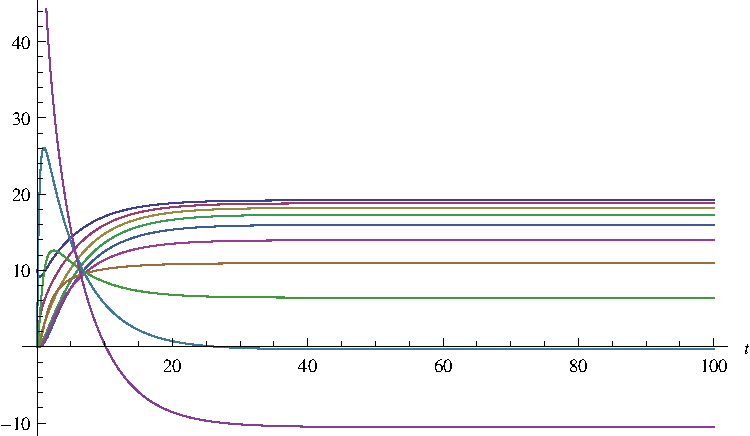
\includegraphics[width=0.8\textwidth]{individual/figures/num_sol_exp_eq_wrong}
    \caption{\label{fig:num_sol_exp_eq_wrong}Numerical solution of
    equations~\eqref{eqn:exp_equation_system_zeroth} with
\(N=10,a=1,b=0.5,c=10,d=10,S_i=0,i=1,\dotsc,N\)}
\end{figure}

\FloatBarrier
\subsection{Analysis of the expectation equations}
The expectation equations for the zeroth order transport process are a
non-closed system. In order to analyse the extent to which the neglection of the
terms relating to the probability of zero particles in
\eqref{eqn:exp_equation_system_zeroth} is a good approximation, we consider a
1-urn pure-death process with death rate \(s H(n)\), where \(n\) is the number
of particles in the urn. This simple process contains many of the difficult
features of the full process. In this case the master equation consists of the
following system:

\begin{align*}
    \diff{p_0}{t} =& s p_1\\
    \diff{p_i}{t} =& s p_{i+1} - s p_i, \quad i = 1,\dotsc,N-1\\
    \diff{p_N}{t} =& - s p_N
\end{align*}
with the initial condition
\begin{equation}
    \label{eqn:pure_death_ic}
    p_i(t=0) = \delta_{iN}.
\end{equation}
This means that there are surely \(N\) particles in the system at \(t=0\). We
are using the notation \(p_n(t)\) to denote the probability of there being \(n\)
particles in the urn at time \(t\).  Analogously to above, the deterministic
mean-field equation can be derived for this process:
\begin{equation*}
    \diff{\E{n}(t)}{t} = -s \left(1-p_0(t)\right).
\end{equation*}
As before, this equation is not closed. Therefore we cannot solve it exactly.
Assuming that \(p_0(t)\) is sufficiently smooth at \(t=0\), we can replace it
with its Taylor series around \(t=0\):
\begin{equation*}
    -s(1-p_0(t)) = -s\left(1 - \left[p_0(0) + \dot{p_0}(0)t +
    \frac{1}{2}\ddot{p_0}(0)t^2 + \dotsb \right] \right).
\end{equation*}

We have that \(p_0(0) = 0\) due to the initial condition. For the second term in
the series,
\begin{equation*}
    \dot{p_0}(0) = \left.(s(p_1)\right|_{t=0} = sp_1(0) = 0.
\end{equation*}
Similarly, for the next term,
\begin{align*}
    \ddot{p_0}(0) &= \left.\left(\diff{}{t}\dot{p_0}\right)\right|_{t=0}\\
    &= \left.\left(\diff{}{t}\left[s p_1\right]\right)\right|_{t=0}\\
    &= s^2\left(p_2(0) - p_1(0)\right) = 0.
\end{align*}
Continuing like this, we find that the derivatives of \(p_0(t)\) follow this
pattern:
\begin{equation*}
    p_0^{(i)}(t) = (-1)^i s^i \sum_{j=0}^{i-1}(-1)^j
    \binom{i-1}{j} p_{1+j}(t),
\end{equation*}
for \(i=1,\dotsc,N-1\).
Due to the initial condition \eqref{eqn:pure_death_ic}, we have that every
derivative is equal to \(0\) for \(i=1,\dotsc,N-1\). The expression for
\(i=N-1\) is
\begin{align*}
    p_0^{(N-1)}(t) &= (-1)^{N-1} s^{N-1} \left\{ p_1(t) - \binom{N-2}{1}p_2(t) +
    \dotsc \right.\\
    &\left.+ (-1)^{N-3} \binom{N-2}{N-3} p_{N-2}(t) +
    (-1)^{N-2}p_{N-1}(t)\right\}.
\end{align*}
Then we have
\begin{align*}
    p_0^{(N)}(t) &= (-1)^{N-1} s^{N-1} \left\{ \dot{p_1}(t) -
    \binom{N-2}{1}\dot{p_2}(t) +
    \dotsc \right.\\
    &\left.+ (-1)^{N-3} \binom{N-2}{N-3} \dot{p_{N-2}}(t) +
    (-1)^{N-2}\dot{p_{N-1}}(t)\right\}\\
    &= (-1)^{N-1} s^{N} \left\{ (p_2-p_1) -
    \binom{N-2}{1}(p_3-p_2) +
    \dotsc \right.\\
    &\left.+ (-1)^{N-3} \binom{N-2}{N-3} (p_{N-1} - p_{N-2}) +
    (-1)^{N-2} (p_N - p_{N-1})\right\}.
\end{align*}
Therefore
\begin{align*}
    p_0^{(N)}(0) &= (-1)^{N-1} (-1)^{N-2} s^N p_N\\
    &= (-1)^{2N-3} s^N
\end{align*}

Putting this together, we find that the Taylor series for \(-s(1-p_0)\) around
\(t=0\) is
\begin{align*}
    -s(1-p_0) = -s\left(1 - \left[ \frac{1}{N!}(-1)^{2N-3}s^N t^N + \dotsb
    \right] \right).
\end{align*}

From this we can see that \(p_0(t)\) grows like \(t^N\). Also, the first term is
scaled by a factor of \(\frac{s^N}{N!}\), which, for large \(N\) is very small.

\section{First order kinetics}
If we now assume that outflow and removal of particles obey first order
kinetics, the transition rates become
\begin{equation}
    \label{eqn:transition_rates_first_order}
    T(\V{n}|\V{n}') =
        \begin{dcases*}
            a n'_{i+1} & for \(\V{n} = \V{n}' + \V{e}_i - \V{e}_{i+1},
            i=1,\dotsc,N-1\)\\
            (a+b) n'_i & for \(\V{n} = \V{n}' - \V{e}_i + \V{e}_{i+1},
            i=1,\dotsc,N-1\)\\
            c & for \(\V{n} = \V{n}' + \V{e}_1\)\\
            d n'_N & for \(\V{n} = \V{n}' - \V{e}_N\)\\
            S_i n'_i & for \(\V{n} = \V{n}' - \V{e}_i, i=1,\dotsc,N\)\\
            0 & otherwise
        \end{dcases*}
\end{equation}
The inflow and hopping rates in remain the same as in
\eqref{eqn:transition_rates_zeroth_order}.
Therefore the only terms that change are those that correspond to removal and
outflow.

\subsection{Jump moments}
In this section we give the first two jump moments \eqref{eqn:jump_moment} for
the first-order transport problem.

\subsubsection{First jump moment}
Starting with \eqref{eqn:jump_moment} and substituting in
\eqref{eqn:transition_rates_first_order} gives
\begin{equation}
    \begin{aligned}
        a_{1i}(\V{n}) =& \sum_{\V{n}'} (n_i' - n_i) T(\V{n}' | \V{n})\\
        &= (1-\delta_{iN})(n_i + 1 - n_i)a n_{i+1}
        +  (1-\delta_{i1})(n_i - 1 - n_i)a n_i\\
        &\quad+ (1-\delta_{iN})(n_i - 1 - n_i)(a+b) n_i
        +  (1-\delta_{i1})(n_i + 1 - n_i)(a+b) n_{i-1}\\
        &\quad+ \delta_{i1}(n_1 + 1 - n_1) c\\
        &\quad+ \delta_{iN}(n_N - 1 - n_N) d n_N\\
        &\quad+ (n_i - 1 - n_i) S_i n_i\\
        &= (1-\delta_{i1})(a+b)n_{i-1} - \left[(2a+b) - \delta_{i1}a -
        \delta_{iN}(a+b) + S_i\right]n_i\\
        &\quad+ (1-\delta_{iN})an_{i+1} + \delta_{i1}c - \delta_{iN}d n_N.
    \end{aligned}
    \label{eqn:first_jump_mom_first_order}
\end{equation}
This is linear in \(\V{n}\) so we have that \eqref{eqn:linear_jump_moments}
holds. Explicitly, we have that the time evolution of the expectation of \(n_i\)
is given by
\begin{equation}
    \begin{aligned}
        \diff{\E{n_i}}{t} &= (1-\delta_{i1})(a+b)\E{n_{i-1}} - \left[(2a+b) -
        \delta_{i1}a - \delta_{iN}(a+b) + S_i\right]\E{n_i}\\
        &\quad+(1-\delta_{iN})a\E{n_{i+1}} + \delta_{i1}c - \delta_{iN}d \E{n_N},
    \end{aligned}
\end{equation}
which is equivalent to the system \eqref{eqn:exp_equation_system_first} given
below.
\begin{subequations}
    \label{eqn:exp_equation_system_first}
    \begin{gather}
        \diff{\V{\E{n}}}{t} = A \V{\E{n}}(t) + \V{b},
        \intertext{where}
        A=
        \begin{pmatrix}
            -(a+b) - S_1 & a & 0 & \dots & \dots & \dots & 0\\
            (a+b)  & -(2a+b) - S_2 & a & 0 & \dots & \dots & 0\\
            \vdots & & \ddots & \ddots & \ddots & & \vdots\\
            0 & \dots & \dots & 0 & (a+b) & -(2a+b) - S_{N-1} & a\\
            0 & \dots & \dots & \dots & 0 & (a+b) & -a -S_N - d
        \end{pmatrix}
        \intertext{and}
        \V{b}=
        \begin{pmatrix}
            c\\
            0\\
            \vdots\\
            0
        \end{pmatrix}
    \end{gather}
\end{subequations}
The coefficients \(\alpha_{1ij}\) (as in \eqref{eqn:linear_jump_moments_coeffs})
are clearly the \(i,j\) elements of the matrix \(A\), and the \(\beta_{1i}\) are the
elements of the vector \(\V{b}\).

\begin{figure}[ht!]
    \centering
    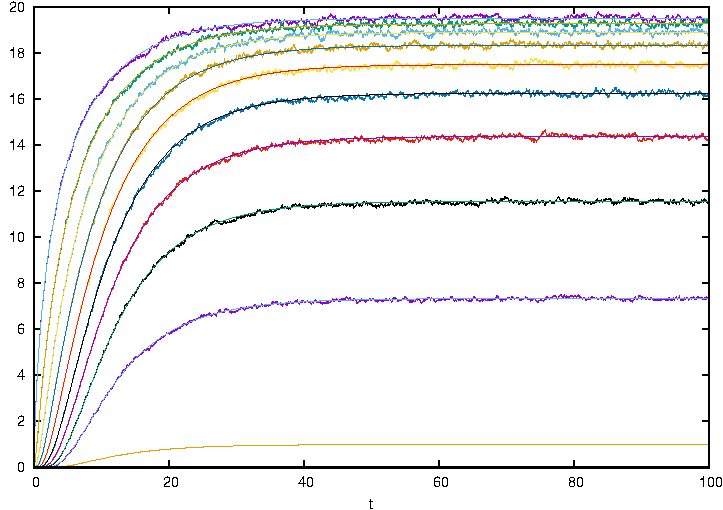
\includegraphics{individual/figures/firstorderrealisation}
    \caption{\label{fig:ex_first_order_real} Comparison between the time evolution of
the sample means of the number of particles in each urn and the mean field
approximation with first order removal kinetics.
\(N=10,a=1,b=0.5,c=10,d=10,S_i=0\).}
\end{figure}

\subsubsection{Second jump moment}
Similarly, we can find the second jump moments:
\begin{equation}
    \begin{aligned}
        a_{2i}(\V{n}) =& \sum_{\V{n}'} (n_i' - n_i)^2 T(\V{n}' | \V{n})\\
        &= (1-\delta_{iN})(n_i + 1 - n_i)^2a n_{i+1}
        +  (1-\delta_{i1})(n_i - 1 - n_i)^2a n_i\\
        &\quad+ (1-\delta_{iN})(n_i - 1 - n_i)^2(a+b) n_i
        +  (1-\delta_{i1})(n_i + 1 - n_i)^2(a+b) n_{i-1}\\
        &\quad+ \delta_{i1}(n_1 + 1 - n_1)^2 c\\
        &\quad+ \delta_{iN}(n_N - 1 - n_N)^2 d n_N\\
        &\quad+ (n_i - 1 - n_i)^2 S_i n_i\\
        &= (1-\delta_{i1})(a+b)n_{i-1} + \left[(2a+b) - \delta_{i1}a -
        \delta_{iN}(a+b) + S_i\right]n_i\\
        &\quad+ (1-\delta_{iN})an_{i+1} + \delta_{i1}c + \delta_{iN}d n_N,
    \end{aligned}
    \label{eqn:second_jump_mom_first_order}
\end{equation}
which is also linear in \(\V{n}\).

We have the following relations between the first and second jump moment
coefficients
\begin{align*}
    \alpha_{1i(i-1)} &= \alpha_{2i(i-1)}\\
    \alpha_{1ii} &= -\alpha_{2ii}\\
    \alpha_{1i(i+1)} &= \alpha_{2i(i+1)}\\
    \beta_{1i} &= \beta_{2i}
\end{align*}

\subsubsection{Mixed jump moments}
Calculating the first mixed jump moment \eqref{eqn:mixed_jump_moment_i_j}
requires slightly more effort than the regular jump moments since every
combination of relations between \(n_i\) and \(n_j\) permitted by the definition
of the rates \eqref{eqn:transition_rates_first_order} must be considered. In the
transport system, particles can only jump from urn \(i\) to urn \(j\) if \(j = i
\pm 1\), which reduces the number of terms we need to consider. However, there
are still many terms; we proceed by considering terms corresponding to each
transition type separately.
\begin{equation}
    a_{1ij}(\V{n}) = \{\text{hop left}\} + \{\text{hop right}\} +
    \{\text{inflow}\} + \{\text{outflow}\} + \{\text{removal}\}
\end{equation}

\begin{align}
    &\begin{aligned}
        \{\text{hop left}\}
        &= \delta_{(i+1)j}(1 - \delta_{iN})(n_i + 1 - n_i)(n_{i+1} - 1 -
        n_{i+1})a n_{i+1}\\
        &+ \delta_{i(j+1)}(1 - \delta_{i1})(n_i - 1 - n_i)(n_{i-1} + 1 -
        n_{i-1})a n_i\\
        &+ \delta_{ij}(1 - \delta_{iN})(n_i + 1 - n_i)(n_i + 1 - n_i)a n_{i+1}\\
        &+ \delta_{ij}(1 - \delta_{i1})(n_i - 1 - n_i)(n_i - 1 - n_i)a n_i
        \label{eqn:mixed_jump_hop_left}
    \end{aligned}\\
    &\begin{aligned}
        \{\text{hop right}\}
        &= \delta_{(i+1)j}(1 - \delta_{iN})(n_i - 1 - n_i)(n_{i+1} + 1 -
        n_{i+1})(a+b) n_i\\
        &+ \delta_{i(j+1)}(1 - \delta_{i1})(n_i + 1 - n_i)(n_{i-1} - 1 -
        n_{i-1})(a+b) n_{i-1}\\
        &+ \delta_{ij}(1 - \delta_{iN})(n_i - 1 - n_i)(n_i - 1 - n_i)(a+b) n_i\\
        &+ \delta_{ij}(1 - \delta_{i1})(n_i + 1 - n_i)(n_i + 1 - n_i)(a+b)
        n_{i-1}
        \label{eqn:mixed_jump_hop_right}
    \end{aligned}\\
    &\begin{aligned}
        \{\text{inflow}\} = \delta_{i1}\delta_{j1} (n_1 + 1 - n_1)(n_1 + 1 -
        n_1)c
        \label{eqn:mixed_jump_inflow}
    \end{aligned}\\
    &\begin{aligned}
        &\{\text{outflow}\} = \delta_{iN}\delta_{jN} (n_N - 1 - n_N)(n_N - 1 - n_N)d
        n_N
        \label{eqn:mixed_jump_outflow}
    \end{aligned}\\
    &\begin{aligned}
        &\{\text{removal}\} = \delta_{ij}(n_i - 1 - n_i)(n_i - 1 - n_i)S_i n_i
        \label{eqn:mixed_jump_removal}
    \end{aligned}
\end{align}
Summing \eqref{eqn:mixed_jump_hop_left}--\eqref{eqn:mixed_jump_removal} and
simplifying gives
\begin{equation}
    \begin{aligned}
        a_{1ij}(\V{n}) &= (a+b)(1-\delta_{i1})(\delta_{ij} -
        \delta_{i(j+1)})n_{i-1}\\
        &+ \left[ a(1-\delta_{i1})(\delta_{ij} -
        \delta_{i(j+1)}) + (a+b)(1-\delta_{iN})(\delta_{ij}-\delta_{(i+1)j}) +
    \delta_{ij}S_i \right]n_i\\
    &+ a(1-\delta_{iN})(\delta_{ij} - \delta_{(i+1)j})n_{i+1} +
    \delta_{i1}\delta_{j1}c + \delta_{jN}\delta_{iN}d n_N
    \end{aligned}
\end{equation}
It is clear from this expression that \(a_{1ij}(\V{n})\) is linear in \(\V{n}\)
and, since \(a_{1i}(\V{n})\) is also linear, we can use the simplified form of
the equation for the covariance \eqref{eqn:time_evo_covar_linear_jump_moments}.

\subsection{Variances}
We are now in a position to write down the equation governing the time
evolution of the variances for the first-order transport problem. Substituting
\eqref{eqn:first_jump_mom_first_order} and
\eqref{eqn:second_jump_mom_first_order} into
\eqref{eqn:time_evo_variance_jump_moment} gives
\begin{equation}
    \begin{aligned}
        \diff{\sigma_i^2}{t} &= (1-\delta_{i1})(a+b)\E{n_{i-1}} +
        \left[(2a+b) - \delta_{i1}a - \delta_{iN}(a+b) + S_i\right]\E{n_i}\\
        &\quad+ (1-\delta_{iN})a\E{n_{i+1}} + \delta_{i1}c + \delta_{iN}d \E{n_N}\\
        &\quad+ 2 \sum_{j=1}^N \alpha_{1ij} \sigma(n_i,n_j)
    \end{aligned}
    \label{eqn:time_evo_variance_first_order}
\end{equation}
So, in general, the variance of \(n_i\) can depend on the covariances between
\(n_i\) and all other \(n_j\). This suggests that we derive the corresponding
equation for the covariances, which we do below.

\subsubsection{No correlation}
If we make the assumption that there is no covariance between any \(n_i, n_j,
i\neq j\), then the equation for the variance simplifies to
\begin{equation}
    \begin{aligned}
        \diff{\sigma_i^2}{t} &= (1-\delta_{i1})(a+b)\E{n_{i-1}} +
        \left[(2a+b) - \delta_{i1}a - \delta_{iN}(a+b) + S_i\right]\E{n_i}\\
        &\quad+ (1-\delta_{iN})a\E{n_{i+1}} + \delta_{i1}c + \delta_{iN}d \E{n_N}\\
        &\quad+ 2 \alpha_{1ii} \sigma_i^2.
    \end{aligned}
    \label{eqn:time_evo_variance_first_order_no_corr}
\end{equation}
This system is only coupled with the other variances, as opposed to
\eqref{eqn:time_evo_variance_first_order} which also depends on the covariances.

\begin{figure}[ht!]
    \centering
    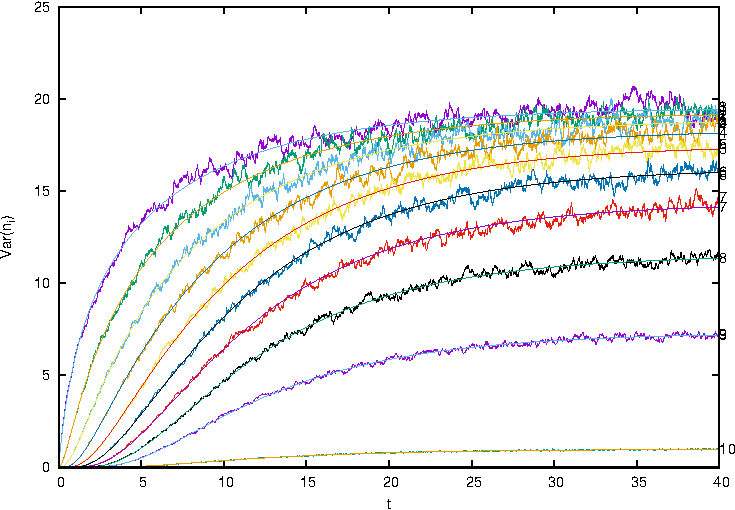
\includegraphics{individual/figures/variance_first_order_no_corr}
    \caption{\label{fig:variance_first_order_no_corr} Comparison of a sample
average of the variance (from 5000 runs) and the analytical prediction under the
assumption zero correlation between urns, with parameters \(N=10,a=1,b=0.5,c=10,d=10,S_i=0\).}
\end{figure}

\subsection{Covariances}
We can now solve \eqref{eqn:time_evo_covar_linear_jump_moments} subject to the
initial conditions
\begin{equation*}
    \sigma_{ij}(t=0) = 0, \text{ for } i,j=1,\dotsc,N.
\end{equation*}
An example solution, given as a matrix plot, is shown in
figure~\ref{fig:ex_covariance_first_order_exact}. For comparison, the
corresponding plot generated from the sample covariances of 9999 Gillespie runs
for the same parameters is shown in
figure~\ref{fig:ex_covariance_first_order_gillespie}.

\begin{figure}
    \centering
    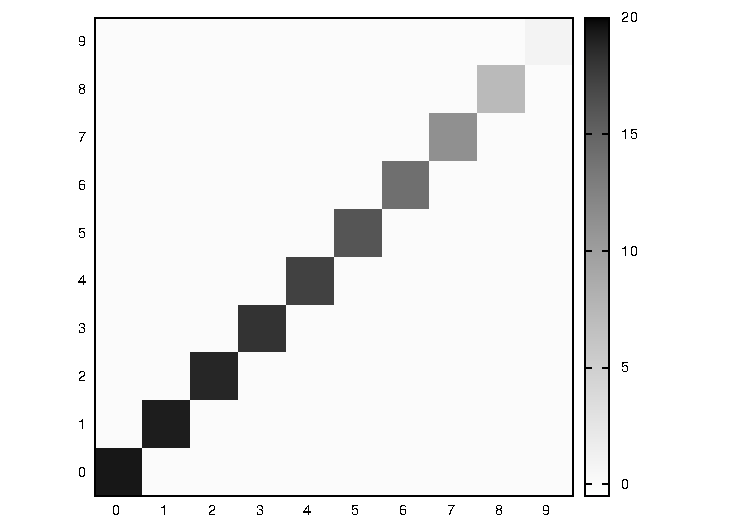
\includegraphics{individual/figures/covariance_exact_40}
    \caption{\label{fig:ex_covariance_first_order_exact}Exact covariance matrix for
parameters \(N=10,a=1,b=0.5,c=10,d=10,S_i=0\)}
\end{figure}
\begin{figure}
    \centering
    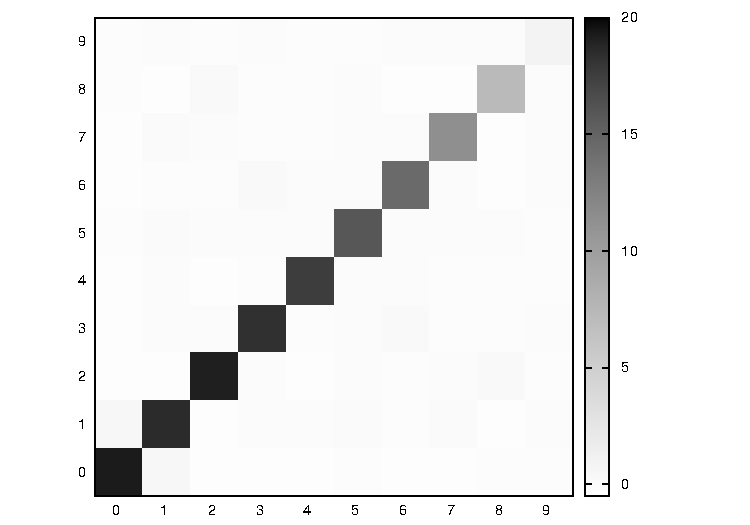
\includegraphics{individual/figures/covariance_gillespie_40}
    \caption{\label{fig:ex_covariance_first_order_gillespie}Sample covariance
matrix (from 9999 runs) for parameters \(N=10,a=1,b=0.5,c=10,d=10,S_i=0\)}
\end{figure}

\todo{plot this in a less terrible way}
\todo{include table of numerical values}

The exact covariance equation \eqref{eqn:time_evo_covar_linear_jump_moments} is
solved numerically using \texttt{Mathematica}. The numerical solution has very
small (\(\sim 10^{-9}\) --- many orders of magnitude smaller than the Gillespie)
off-diagonal elements which are most likely numerical artefacts.

\FloatBarrier
\section{Todo/problems}
\begin{itemize}
    \item Show analytically that \(\sigma_{ij} = 0\) when \(i \neq j\)
    \item Write up exact solution of 1 urn 1st order death process
    \item Unbiased transport --- keep biased everywhere except for when solving
        the linear system?
    \item Update plots --- consistent colours, line labels
\end{itemize}

\chapter{Continuum approach}
\section{Identical sinks}

The distribution of the concentration \(C(x)\) of a solute in a constant,
uniform, unidirectional flow \(u_0\) in a domain of length \(L\) containing
\(N\) identical point sinks of constant strength \(q_0\) is governed by the
one-dimensional advection-diffusion equation,
\begin{subequations}
    \label{eqn:nondim_advec_diff}
    \begin{gather}
        \label{eqn:nondim_advec_diff_eq}
        \Pe C_x - C_{xx} = - \Da f(x), \text{ for } 0 < x < \varepsilon^{-1},\\
        \label{eqn:nondim_advec_diff_bcs}
        C(0) = 1, \quad C(\varepsilon^{-1}) = 0,
    \end{gather}
\end{subequations}
where \(\Pe=u_0 l/D\) is the Péclet number, \(\Da=q_0 l/(D C_0)\) is the
Damköhler number and the sink distribution is given by
\begin{equation}
    \label{eqn:point_sink_dist}
    f(x) = \sum_{i=1}^{N} \delta(x-\xi_i).
\end{equation}
The ordered sink locations \(0 < \xi_1 < \cdots < \xi_N < L\) must be sampled
from a distribution, either a periodic distribution, i.e. \(\xi_i=i,
\Delta_i=1\), where \(\Delta_i = \xi_i - \xi_{i-1}\), for \(1\le\xi\le N\), or
some random distribution (TODO). For convenience, define \(\xi_0 = 0\) and
\(\xi_{N+1} = \varepsilon^{-1}\).

Regardless of the distribution of the sink locations, the solution between any
two sinks (including the boundary points \(\xi_0, \xi_{N+1}\)), say \(\xi_i,
\xi_{i+1}\), is of the following form,
\begin{gather}
    \label{eqn:gen_sol_piece}
    C_i(x)=A_i e^{\Pe x}+B_i\\
    \text{ for } \xi_i \le x \le \xi_{i+1}, \text{ for } 0 \le i \le N.
\end{gather}

To determine the constants \(A_i, B_i\), we must apply the boundary conditions
of the problem to the general solution.

The boundary conditions~\eqref{eqn:nondim_advec_diff_bcs} imply
\begin{equation}
    \label{eqn:bc_A_0_B_0}
    C_0(0) = A_0 + B_0 = 1,
\end{equation}
and
\begin{equation}
    \label{eqn:bc_A_N_B_N}
    C_N(1) = A_N e^{\Pe} + B_N = 0.
\end{equation}

However, to fully determine the coefficients we must first obtain the
conditions on the flux of concentration at the locations of the sinks. To do
this for the sink at \(\xi_i\), say, we integrate
equation~\eqref{eqn:nondim_advec_diff_eq} over the interval
\([\xi_i-\alpha,\xi_i+\alpha]\), and take the limit as \(\alpha \to 0\):
\begin{align*}
    \lim_{\alpha \to 0}
    \int_{\xi_i-\alpha}^{\xi_i+\alpha}\left(\Pe C_x - C_{xx}\right)\dd x = &
    \lim_{\alpha \to 0}
    \Big[\Pe C - C_x\Big]_{\xi_i-\alpha}^{\xi_i+\alpha}\\
    = & C_x^-(\xi_i) - C_x^+(\xi_i)\\
    = & -\lim_{\alpha \to 0}
    \int_{\xi_i-\alpha}^{\xi_i+\alpha}\Da f(x) \dd x\\
    = & - \Da,
\end{align*}
where we have applied the condition that the concentration \(C(x)\) is
continuous everywhere, and standard properties of the Dirac delta function.
Therefore, the flux of the concentration decreases by the Damköhler
number \(\Da\) at each sink.

We can then apply the flux condition to equation~\eqref{eqn:gen_sol_piece} for
the two pieces of the solution that meet at the sink at \(\xi_i\):
\(C_{i-1}(x)\) and \(C_i(x)\).
\begin{equation*}
    %\nonumber
    {C_{i-1}}_x(\xi_i) = {C_i}_x(\xi_i) - \Da,%\\
    %\nonumber
    %\implies & \Pe A_{i-1} e^{\Pe \xi_i} = \Pe A_i e^{\Pe \xi_i} - \Da\\
\end{equation*}
which gives after substitution
\begin{equation}
    \label{eqn:bc_A_i}
    A_i = A_{i-1} + \frac{e^{-\Pe \xi_i}\Da}{\Pe}.
\end{equation}
Applying \eqref{eqn:bc_A_i} to itself recursively gives an expression for
\(A_i\) in terms of the sinks locations and \(A_0\):
\begin{equation}
    \label{eqn:A_i}
    %\boxed{
    A_i = A_0 + \frac{\Da}{\Pe}\sum_{j=1}^{i} e^{-\Pe \xi_j}
    %}
\end{equation}
Similarly, continuity of concentration across the sink at \(\xi_i\) gives
\begin{equation*}
    %\nonumber
    C_{i-1}(\xi_i) = C_i(\xi_i),
\end{equation*}
and so
\begin{equation}
    %\nonumber
    %\implies & A_{i-1} e^{\Pe \xi_i} + B_{i-1} = A_i e^{\Pe \xi_i} + B_i\\
    %\nonumber
    %\implies & A_{i-1} e^{\Pe \xi_i} + B_{i-1} = \frac{\Da}{\Pe} + A_{i-1}
    %e^{\Pe \xi_i} + B_i\\
    \label{eqn:bc_B_i}
    B_i = B_{i-1}-\frac{\Da}{\Pe}.
\end{equation}
As above, applying \eqref{eqn:bc_B_i} recursively gives an expression for
\(B_i\):
\begin{equation}
    \label{eqn:B_i}
    %\boxed{
    B_i = B_0 - i\frac{\Da}{\Pe}.
    %}
\end{equation}
Applying \eqref{eqn:bc_B_i} to \eqref{eqn:bc_A_0_B_0} \(N\) times gives
\begin{equation}
    \label{eqn:bc_A_0_B_N}
    A_0 + N \frac{\Da}{\Pe} + B_N = 1.
\end{equation}
Now use \eqref{eqn:bc_A_N_B_N} with \eqref{eqn:bc_A_0_B_N} to obtain
\begin{equation}
    \label{eqn:bc_A_0_A_N}
    A_0 + N \frac{\Da}{\Pe} - A_N e^{\Pe \varepsilon^{-1}} = 1.
\end{equation}
Applying \eqref{eqn:bc_A_i} to \eqref{eqn:bc_A_0_A_N} \(N\) times and
rearranging gives
\begin{equation}
    %\nonumber
    %& A_0 + N \frac{\Da}{\Pe} - e^{\Pe \varepsilon^{-1}}
    %\left(A_0 + \frac{\Da}{\Pe} \sum_{i=1}^{N}e^{-\Pe \xi_i}\right) = 1\\
    %\nonumber
    %\implies & \left(1 - e^{\Pe \varepsilon^{-1}}\right) A_0 +
    %\frac{\Da}{\Pe} \left(N - e^{\Pe \varepsilon^{-1}} \sum_{i=1}^{N} e^{-\Pe
    %\xi_i}\right) = 1\\
    %\implies & \boxed{
    \label{eqn:A_0}
    A_0 = \frac{1 -
    \frac{\Da}{\Pe} \left(N - e^{\Pe \varepsilon^{-1}} \sum_{i=1}^{N} e^{-\Pe
    \xi_i}\right)}{1 - e^{\Pe \varepsilon^{-1}}}.
    %}
\end{equation}
Similarly, \eqref{eqn:A_0} and \eqref{eqn:bc_A_0_B_0} give
\begin{equation}
    %\boxed{
    \label{eqn:B_0}
    B_0 = 1 - \frac{1 -
    \frac{\Da}{\Pe} \left(N - e^{\Pe \varepsilon^{-1}} \sum_{i=1}^{N} e^{-\Pe
    \xi_i}\right)}{1 - e^{\Pe \varepsilon^{-1}}}.
    %}
\end{equation}

\begin{figure}[ht!]
    \centering
    \begin{subfigure}[b]{0.45\textwidth}
        \centering
        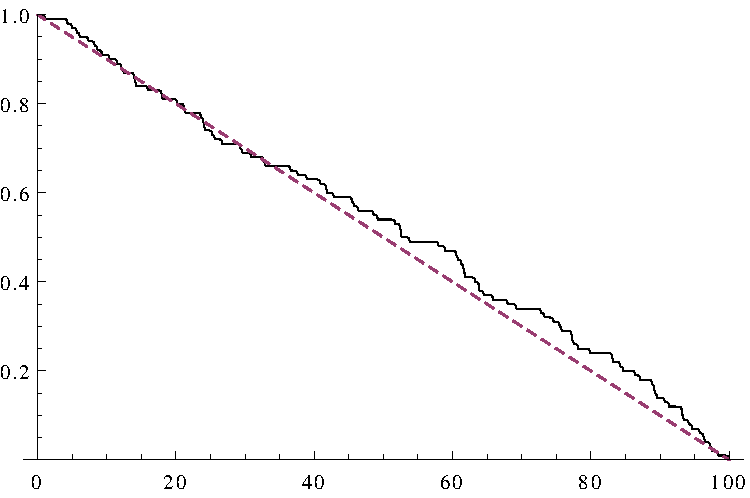
\includegraphics[scale=0.5]{continuum/figures/loc_uniform_dist/1}
    \end{subfigure}
    \begin{subfigure}[b]{0.45\textwidth}
        \centering
        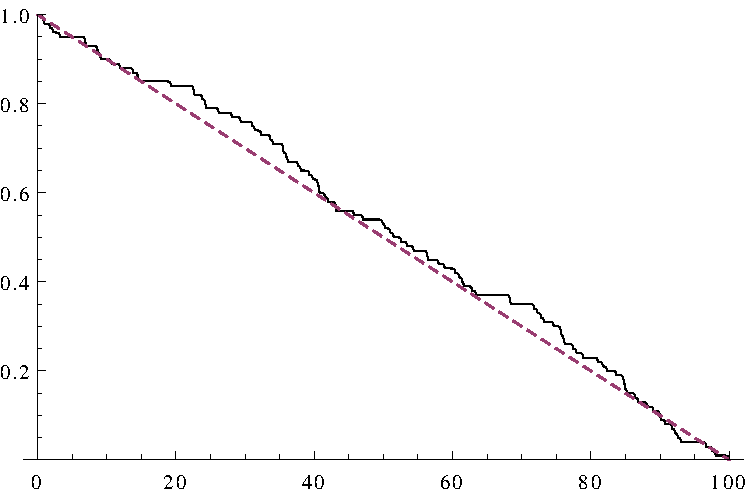
\includegraphics[scale=0.5]{continuum/figures/loc_uniform_dist/2}
    \end{subfigure}
    \\
    \begin{subfigure}[b]{0.45\textwidth}
        \centering
        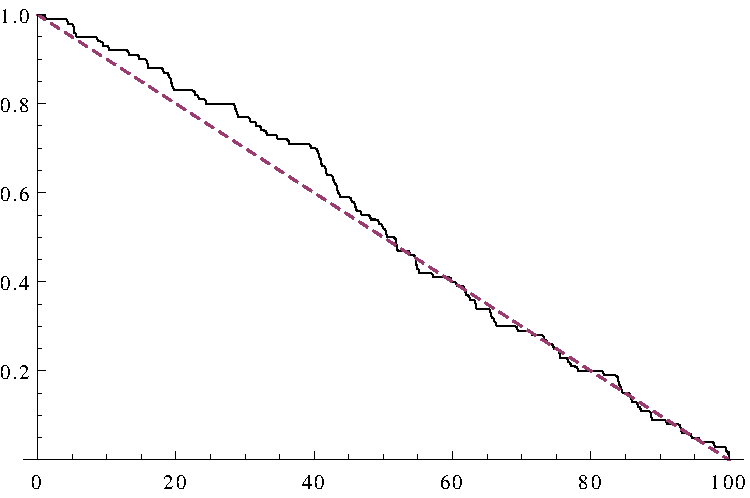
\includegraphics[scale=0.5]{continuum/figures/loc_uniform_dist/3}
    \end{subfigure}
    \begin{subfigure}[b]{0.45\textwidth}
        \centering
        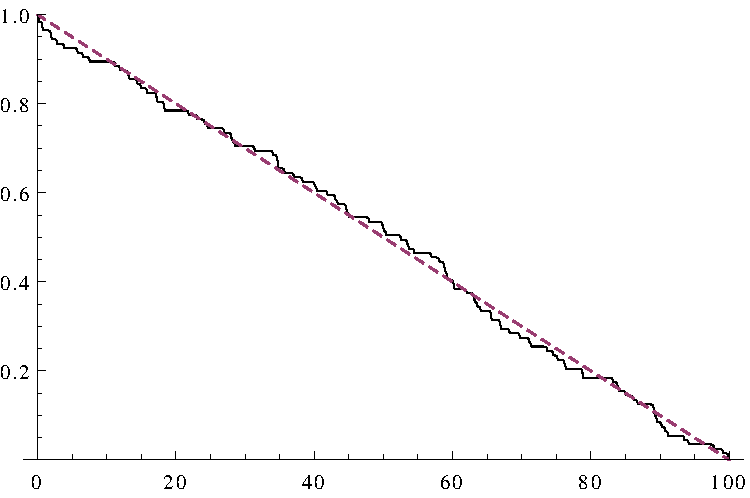
\includegraphics[scale=0.5]{continuum/figures/loc_uniform_dist/4}
    \end{subfigure}
    \caption{\label{fig:99_sinks_uni_pos}Four realisations of 99 sinks with
    uniformly random positions and
        \({\Pe=10}, {\Da=\varepsilon\Pe}\)}
\end{figure}

\FloatBarrier

\subsubsection{Sample statistics}
We define the homogenisation residue as
\begin{equation}
    \label{eqn:homogenisation_residue}
    r^\varepsilon(X) = C - C^{(0)}.
\end{equation}

In the regime \(\Pe = \bo{\varepsilon}, \Da = \bo{\varepsilon^2}\), the
first order homogenisation approximation is \(C^{(0)}(X) = 1 - X\). We will use
the residue to compare realisations of concentration distributions to the first
order approximation.

Figure~\ref{fig:loc_uniform_1000_av_residuals} shows the sample mean and
variance (scaled by a factor of \(\varepsilon^{-1}\) *is there a mathematical
reason for the scalings in the papers or are they graphically convenient? This
one is the latter\ldots*) of
\(r^\varepsilon\) computed from 1000 realisations of the uniformly random sink
locations.

\begin{figure}[ht!]
    \centering
    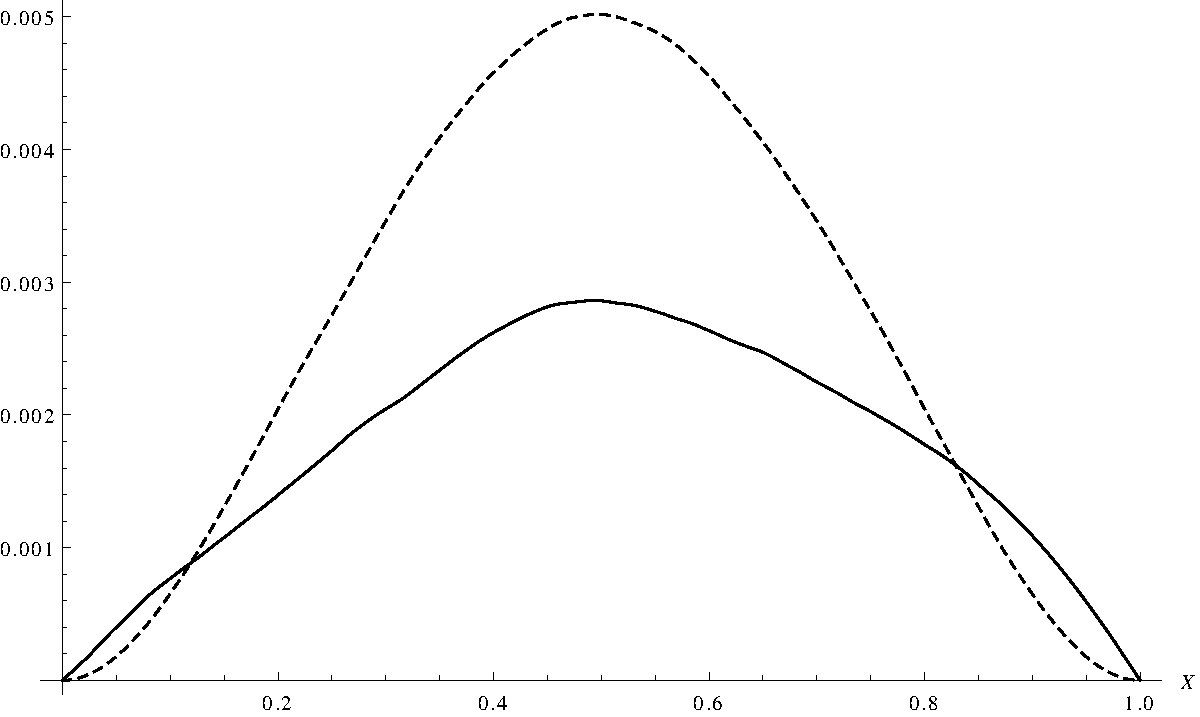
\includegraphics[width=0.9\textwidth]{continuum/figures/loc_uniform_dist/av_res_var_1000_samples}
    \caption{\label{fig:loc_uniform_1000_av_residuals}Pointwise sample mean
    (solid) and variance (dashed; scaled by \(\varepsilon^{-1}\)) of
    \(r^\varepsilon\) calculated from 1000 Monte Carlo samples for uniformly
    distributed sinks with constant (unit) strength with, \({\Pe=\varepsilon},
    {\Da=\varepsilon\Pe}\)}
\end{figure}

\FloatBarrier

\section{Sinks of varying strength}

We now allow the sinks to have different strengths. The solution between each
pair of sinks has the same form (\(C_i(x)=A_i e^{\Pe x} + B_i\)) but the
coefficients \(A_i\) and \(B_i\) will change. Let \(q_i\) be the
(nondimensional --- \(q_0\) can now be thought of as the mean sink strength
against which the strengths are nondimensionalised) strength of sink \(\xi_i\).
Going through the calculations equivalent to the above yields the following
expressions for the coefficients:
\begin{equation}
    \label{eqn:varying_strength_A_0}
    %\boxed{
    A_0 = \frac{1 -
        \frac{\Da}{\Pe} \sum_{i=1}^N q_i \left(1 - e^{\Pe(\varepsilon^{-1}
        -\xi_i)}\right)}{1 - e^{\Pe \varepsilon^{-1}}},
    %}
\end{equation}
\begin{equation}
    \label{eqn:varying_strength_B_0}
    %\boxed{
    B_0 = 1 - \frac{1 -
        \frac{\Da}{\Pe} \sum_{i=1}^N q_i \left(1 - e^{\Pe(\varepsilon^{-1}
        -\xi_i)}\right)}{1 - e^{\Pe \varepsilon^{-1}}},
    %}
    %\boxed{B_0 = 1 - \frac{1 -
    %    \frac{\Da}{\Pe} \left(\sum_{i=1}^N q_i - e^{\Pe \varepsilon^{-1}}
    %    \sum_{i=1}^{N} q_i e^{-\Pe
    %    \xi_i}\right)}{1 - e^{\Pe \varepsilon^{-1}}},}
\end{equation}
\begin{equation}
    \label{eqn:varying_strength_A_i}
    %\boxed{
    A_i = A_0 + \frac{\Da}{\Pe}\sum_{j=1}^i q_j e^{-\Pe \xi_j},
%}
\end{equation}
\begin{equation}
    \label{eqn:varying_strength_B_i}
    %\boxed{
    B_i = B_0 - \frac{\Da}{\Pe} \sum_{j=1}^i q_j.
%}
\end{equation}

\subsection{Log-normally distributed sink strengths}
If a random variable \(X\) is normally distributed, then \(Y=\exp(X)\) is
log-normally distributed, denoted by \(Y\sim\ln\mathcal{N}(\mu,\sigma^2)\). The
parameters \(\mu,\sigma^2\) are the mean and variance of the corresponding
normal distribution, \(\mathcal{N}(\mu,\sigma^2)\). They are related to the mean
\(m\) and variance \(v\) of the log-normal distribution by
\begin{gather*}
    \mu = \ln\left(\frac{m^2}{\sqrt{v+m^2}}\right)\\
    \sigma = \sqrt{\ln\left(1+\frac{v}{m^2}\right)}
\end{gather*}

\begin{figure}[ht!]
    \centering
    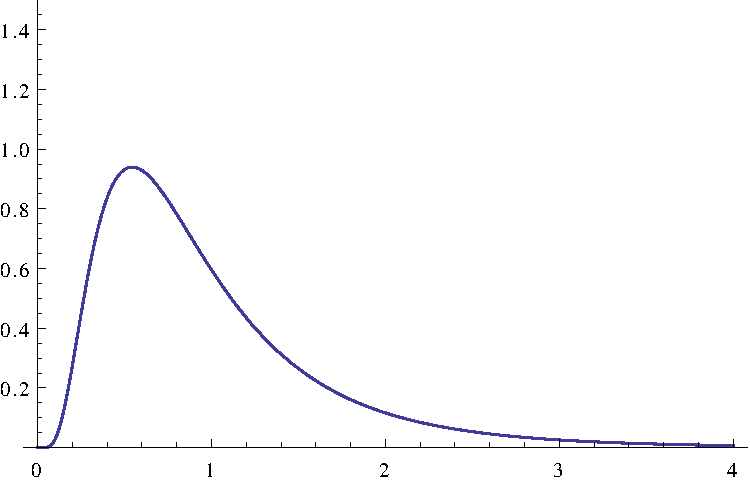
\includegraphics[width=0.7\textwidth]{continuum/figures/log_normal_pdf}
    \caption{\label{fig:log_normal_pdf}PDF of the log-normal distribution with mean 1 and variance 0.5}
\end{figure}

\FloatBarrier

\begin{figure}[ht!]
    \centering
    \begin{subfigure}[b]{0.45\textwidth}
        \centering
        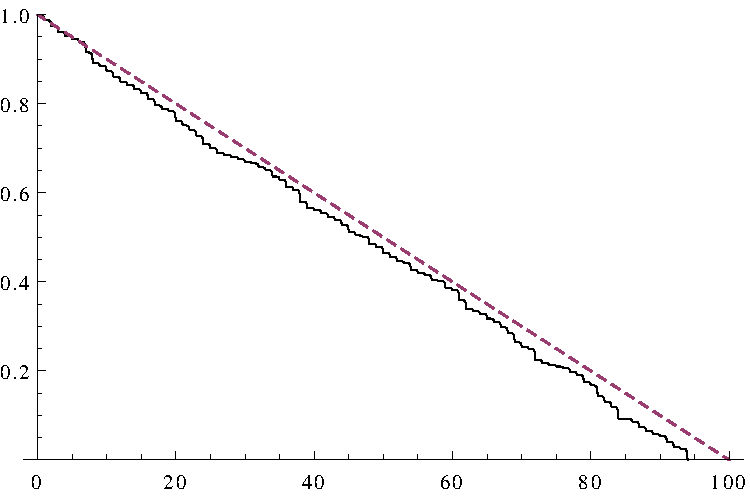
\includegraphics[scale=0.5]{continuum/figures/strength_lognormal_dist/1}
    \end{subfigure}
    \begin{subfigure}[b]{0.45\textwidth}
        \centering
        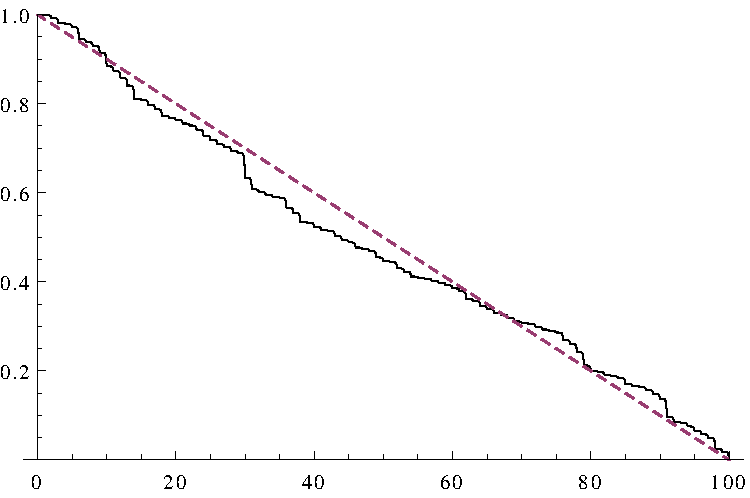
\includegraphics[scale=0.5]{continuum/figures/strength_lognormal_dist/2}
    \end{subfigure}
    \\
    \begin{subfigure}[b]{0.45\textwidth}
        \centering
        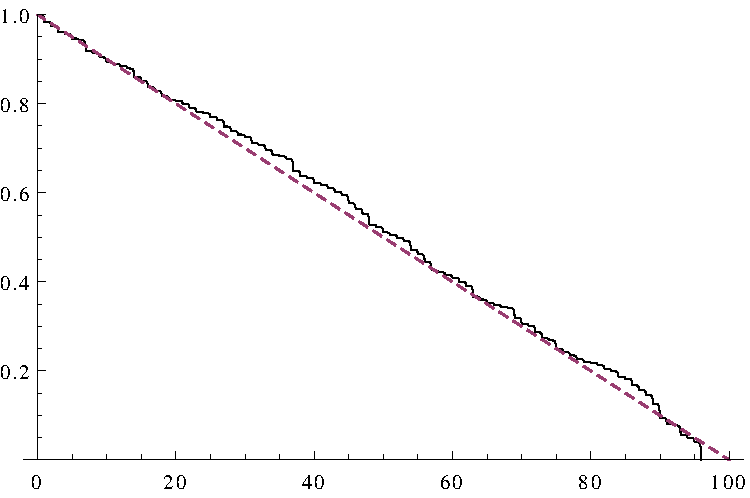
\includegraphics[scale=0.5]{continuum/figures/strength_lognormal_dist/3}
    \end{subfigure}
    \begin{subfigure}[b]{0.45\textwidth}
        \centering
        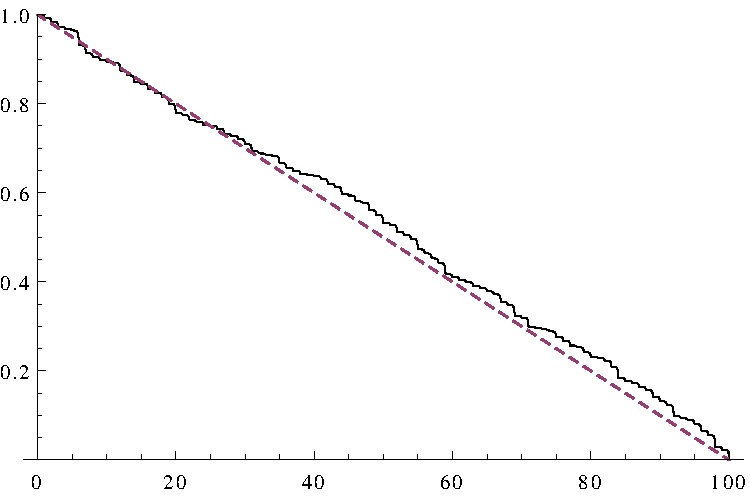
\includegraphics[scale=0.5]{continuum/figures/strength_lognormal_dist/4}
    \end{subfigure}
    \caption{\label{fig:99_sink_periodic_pos}Four realisations of 99 sinks with
    periodic positions and log-normally distributed strengths \({m=1}, {v=0.5},
    {\Pe=10}, {\Da=\varepsilon\Pe}\)}
\end{figure}

\FloatBarrier

\subsubsection{Sample statistics}

Figure~\ref{fig:log_normal_1000_av_residuals} shows the pointwise sample mean of
the residual \(r^\varepsilon = C - C^{(0)}\) for log-normally distributed sink
strengths and periodic sink positions.

%Since the mean of the log normal
%distribution used for the sink strengths is 1, one might expect (after
%performing many trials) the sample mean residuals to be close to those of the
%case of periodic sink positions and unit sink strengths. The figure, generated
%from 1000 samples, supports this.

\begin{figure}[ht!]
    \centering
    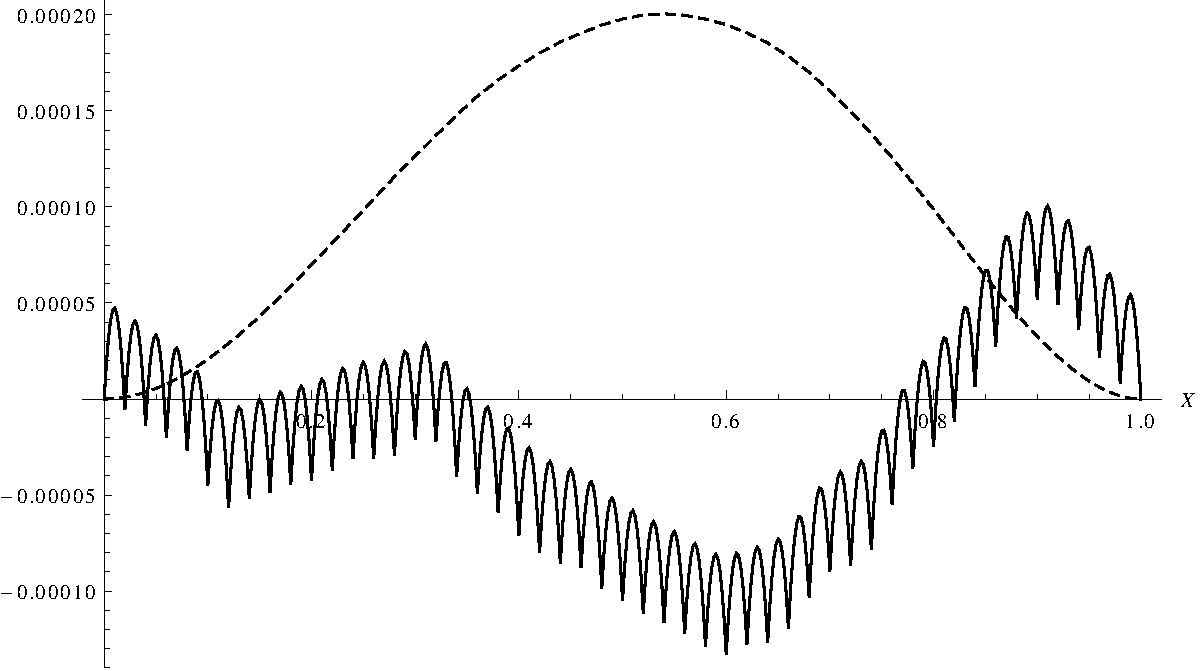
\includegraphics[width=0.9\textwidth]{continuum/figures/strength_lognormal_dist/av_res_var_1000_samples}
    \caption{\label{fig:log_normal_1000_av_residuals}Pointwise sample mean
    (solid) and variance (dashed) of \(r^\varepsilon\) calculated from
    1000 Monte Carlo samples for log-normally distributed sink strengths with
    \({m=1}, {v=0.5},
    {\Pe=\varepsilon}, {\Da=\varepsilon\Pe}\)}
\end{figure}

\FloatBarrier

\section{Homogenisation for periodically distributed sinks}

We will be applying the method of homogenisation to equations
\eqref{eqn:nondim_advec_diff} and \eqref{eqn:point_sink_dist} in the case where
the sink locations are periodically distributed, i.e. \(\xi_i = i, 1 \le i \le
N\). The motivation for this approach is the observation that there are features
of the solution \(C(x)\) that occur on different characteristic length scales.
For example, in figure~\ref{fig:99_sink_periodic_pos}, one can see that over the
length of the whole domain, there is a steady decrease in the concentration. In
addition, on the scale of the (nondimensional) distance between adjacent sinks,
\(\varepsilon\), there is a rapid change in concentration near each sink, and
the concentration then levels off until it approaches another sink. The idea of
homogenisation is to use a multiple scales expansion to capture the variations
on both length scales separately by introducing an additional variable, treated
as independent of \(x\) (technically one that tends to independence from \(x\)
as \(\varepsilon \to 0\) in a weak two-scale sense).  Then, there is usually an
averaging step over the small length scale in order to be able to extract the
approximate ``average'' behaviour over the whole domain.

We will seek solutions to \eqref{eqn:nondim_advec_diff} and
\eqref{eqn:point_sink_dist} of the form
\begin{equation}
    \label{eqn:C(x,X)}
    C(x) = \ti{C}(x,X),
\end{equation}
where we define \(X = \varepsilon x\) to be the ``slow'' variable. \(x\) is
referred to as the ``fast'' variable. The derivative with respect to \(x\)
transforms to
\begin{equation}
    \label{eqn:x_deriv_fast_slow}
    \diff{}{x} = \pdiff{}{x} + \varepsilon\pdiff{}{X},
\end{equation}
where we have ``reused'' the variable name \(x\) to simplify notation.
Henceforth, subscripts will denote partial derivatives (now that \(x\)
and \(X\) are being treated as independent).

Substituting \eqref{eqn:x_deriv_fast_slow} into
equation~\eqref{eqn:nondim_advec_diff} gives
\begin{subequations}
    \label{eqn:nondim_advec_diff_x_X}
    \begin{gather}
        \label{eqn:nondim_advec_diff_eq_x_X}
        \Pe\left(\ti{C}_x + \varepsilon\ti{C}_X\right) = \ti{C}_{xx}
        + 2\varepsilon\ti{C}_{xX} + \varepsilon^2\ti{C}_{XX} - \Da f(x),\\
        \nonumber \text{for } 0 \le x \le \varepsilon^{-1}\\
        \label{eqn:nondim_advec_diff_bcs_x_X}
        \left.\ti{C}\right|_{X=0} = 1, \quad \left.\ti{C}\right|_{X=1} = 0.
    \end{gather}
\end{subequations}
The orders of the Péclet and Damköhler numbers will therefore affect which terms
appear at each order of the problem, and so we must specify their orders before
solving. Additionally, we assume that \(\ti{C}(x,X)\) is \(x\)-periodic with
period \(1\). This represents the fact that we expect the local effect of each
sink on the concentration to be identical, so that the concentration only
depends on the position of sinks.

We can simplify this by solving only between each pair of adjacent sinks, and
introducing a condition at each sink to handle the jump in flux, so that
\(f(x)\) no longer appears explicitly:
\begin{subequations}
    \label{eqn:nondim_advec_diff_eq_x_X_no_f}
    \begin{gather}
        \Pe\left(\ti{C}_x + \varepsilon\ti{C}_X\right) = \ti{C}_{xx},
        + 2\varepsilon\ti{C}_{xX} + \varepsilon^2\ti{C}_{XX},\\
        \nonumber \text{for } x \ne i,\\
        \jump{\ti{C}_x + \varepsilon \ti{C}_X}_{x=i},\\
        \left.\ti{C}\right|_{X=0} = 1, \quad \left.\ti{C}\right|_{X=1} = 0,\\
        \nonumber i = 1, \dotsc, N.
    \end{gather}
\end{subequations}

We will seek approximate solutions to \eqref{eqn:nondim_advec_diff_eq_x_X_no_f}
of the form
\begin{equation}
    \label{eqn:x_X_asymptotic_expansion}
    C(x) = \ti{C}(x,X) = C^{(0)}(x,X) + \varepsilon C^{(1)}(x,X) + \varepsilon^2
    C^{(2)}(x,X) + \dotsb.
\end{equation}

\subsection{\(\Pe = \bo{\varepsilon}, \Da = \bo{\varepsilon^2}\)}
\label{sec:0th-order,Pe=O(e),Da=O(e^2)}

We now set \(\Pe = \varepsilon p, \Da = \varepsilon^2 q\), where \(p, q =
\bo{1}\) as \(\varepsilon \to 0\). Substituting these definitions and
\eqref{eqn:x_X_asymptotic_expansion} into
\eqref{eqn:nondim_advec_diff_eq_x_X_no_f} gives
\begin{subequations}
    \label{eqn:full_Pe=O(e),Da=O(e^2)}
    \begin{gather}
        \begin{gathered}
            p \left(
            \varepsilon C^{(0)}_x + \varepsilon^2 C^{(1)}_x + \dotsb +
            \varepsilon^2 C^{(0)}_X + \varepsilon^3 C^{(1)}_x + \dotsb \right) =
            C^{(0)}_{xx} + \varepsilon C^{(1)}_{xx} + \dotsb\\
            + 2\left(\varepsilon C^{(0)}_{xX} + \varepsilon^2 C^{(1)}_{xX} +
            \dotsb \right) +
            \varepsilon^2 C^{(0)}_{XX} + \varepsilon^3 C^{(1)}_{XX} + \dotsb,
        \end{gathered}\\
        \nonumber \text{for } x \ne i,\\
        \jump{C^{(0)}_x + \varepsilon C^{(1)}_x + \dotsb + \varepsilon C^{(0)}_X
        + \varepsilon^2 C^{(1)}_X + \dotsb}_{x=i} = \varepsilon^2 q,\\
        \left.\left(C^{(0)} + \varepsilon C^{(1)} + \dotsb\right)\right|_{X=0}
        = 1,\\
        \left.\left(C^{(0)} + \varepsilon C^{(1)} + \dotsb\right)\right|_{X=1}
        = 0,\\
        \nonumber i = 1, \dotsc, N.
    \end{gather}
\end{subequations}
We proceed by collecting terms by order in \(\varepsilon\). We also exploit the
\(x\)-periodicity of \(\ti{C}(x,X)\) by only solving in the sub-domain
\(-1/2 < x < 1/2\), representing a unit cell surrounding a sink, with the
sink at \(x = 0\). This only affects the jump conditions --- clearly
the governing equation is invariant under a translation in \(x\).

At \(\bo{1}\):
\begin{subequations}
    \label{eqn:O(1),Pe=O(e),Da=O(e^2)}
    \begin{gather}
        \label{eqn:O(1)_eqn,Pe=O(e),Da=O(e^2)}
        C^{(0)}_{xx} = 0,\\
        \label{eqn:O(1)_jump_cond,Pe=O(e),Da=O(e^2)}
        \jump{C^{(0)}}_{x=0}=0, \quad \jump{C^{(0)}_x}_{x=0}=0,\\
        \label{eqn:O(1)_bcs,Pe=O(e),Da=O(e^2)}
        \left.C^{(0)}\right|_{X=0}=1, \quad \left.C^{(0)}\right|_{X=1}=0.
    \end{gather}
\end{subequations}
Integrating \eqref{eqn:O(1)_eqn,Pe=O(e),Da=O(e^2)} gives
\begin{equation}
    \label{}
    C^{(0)}(x,X) = \ti{A}_0(X)x + \ti{B}_0(X),
\end{equation}
where \(\ti{A}_0(X),\ti{B}_0(X)\) are arbitrary functions. Since the full
domain of \(x\) is \((0,\varepsilon^{-1})\), we must suppress the first term by
setting \(\ti{A}_0 \equiv 0\). This is to avoid secular (unbounded) growth in
\(C^{(0)}\) as \(\varepsilon \to 0\). Therefore, we have that \(C^{(0) } =
C^{(0)}(X)\) only. An interpretation of this is that at a first approximation,
the behaviour of the concentration is governed solely by the boundary
conditions on the ends of the domain.

At \(\bo{\varepsilon}\):
\begin{subequations}
    \label{eqn:O(e),Pe=O(e),Da=O(e^2)}
    \begin{gather}
        \label{eqn:O(e)_eqn,Pe=O(e),Da=O(e^2)}
        C^{(1)}_{xx} = 0,\\
        \label{eqn:O(e)_jump_cond,Pe=O(e),Da=O(e^2)}
        \jump{C^{(1)}}_{x=0}=0, \quad \jump{C^{(1)}_x}_{x=0}=0,\\
        \label{eqn:O(e)_bcs,Pe=O(e),Da=O(e^2)}
        \left.C^{(1)}\right|_{X=0}=0, \quad \left.C^{(1)}\right|_{X=1}=0.
    \end{gather}
\end{subequations}
By the same reasoning as above, we find that \(C^{(1)} = C^{(1)}(X)\) only.
*Not clear on the justification for the next step* We further find that
\(C^{(1)} \equiv 0\).

At \(\bo{\varepsilon^2}\):
\begin{subequations}
    \label{eqn:O(e^2),Pe=O(e),Da=O(e^2)}
    \begin{gather}
        \label{eqn:O(e^2)_eqn,Pe=O(e),Da=O(e^2)}
        p C^{(0)}_X = C^{(2)}_{xx} + C^{(0)}_{XX},\\
        \label{eqn:O(e^2)_jump_cond,Pe=O(e),Da=O(e^2)}
        \jump{C^{(2)}}_{x=0}=0, \quad \jump{C^{(2)}_x}_{x=0}=q,\\
        \label{eqn:O(e^2)_bcs,Pe=O(e),Da=O(e^2)}
        \left.C^{(2)}\right|_{X=0}=0, \quad \left.C^{(2)}\right|_{X=1}=0.
    \end{gather}
\end{subequations}
This is the lowest order at which we have seen interaction between advection,
diffusion and uptake. We now integrate equation
\eqref{eqn:O(e^2)_eqn,Pe=O(e),Da=O(e^2)} over the unit cell:
\begin{align}
    \label{eqn:averaged_over_unit_cell,Pe=O(e),Da=O(e^2)}
    \nonumber &\left(\lim_{\delta \to 0^-} \int_{-1/2}^{\delta}\dd x +
    \lim_{\delta \to 0^+} \int_{\delta}^{1/2}\dd x\right)
    \left(p C^{(0)}_X - C^{(0)}_{XX} - C^{(2)}_{xx} \right) = 0\\
    \nonumber \implies & \left[x\right]_{-1/2}^{1/2}\left(p C^{(0)}_X -
    C^{(0)}_{XX}\right)\\
    & = p C^{(0)}_X - C^{(0)}_{XX}
    = \left.C^{(2)}_x\right|_{1/2} - \left.C^{(2)}_x\right|_{-1/2}
    -\jump{C^{(2)}_x}_{x=0}.
\end{align}
Using the assumption of periodcitiy of \(C^{(2)}_x\) in the unit cell,
equation~\eqref{eqn:averaged_over_unit_cell,Pe=O(e),Da=O(e^2)} becomes, using
the conditions~\eqref{eqn:O(e^2)_jump_cond,Pe=O(e),Da=O(e^2)}, an
advection-diffusion equation for \(C^{(0)}\):
\begin{subequations}
    \label{eqn:O(1)_averaged,Pe=O(e),Da=O(e^2)}
    \begin{gather}
        \label{eqn:O(1)_averaged_eqn,Pe=O(e),Da=O(e^2)}
        C^{(0)}_{XX} - p C^{(0)}_X = q,\\
        \label{eqn:O(1)_averaged_bcs,Pe=O(e),Da=O(e^2)}
        \left.C^{(0)}\right|_{X=0}=1, \quad \left.C^{(0)}\right|_{X=1}=0,
    \end{gather}
\end{subequations}
The solution of \eqref{eqn:O(1)_averaged,Pe=O(e),Da=O(e^2)} is
\begin{equation}
    \label{eqn:C^0(X)_solution,Pe=O(e),Da=O(e^2)}
    C^{(0)}(X) = \left(\frac{q}{p} - 1\right)\frac{e^{pX} - 1}{e^{p} - 1} -
    \frac{q}{p}X + 1
\end{equation}
Substituting \eqref{eqn:O(1)_averaged_eqn,Pe=O(e),Da=O(e^2)} into
\eqref{eqn:O(e^2)_eqn,Pe=O(e),Da=O(e^2)} gives the equation that \(C^{(2)}(X)\)
must satisfy:
\begin{equation}
    \label{eqn:O(e^2)_actual,Pe=O(e),Da=O(e^2)}
    C^{(2)}_{xx} = -q, \quad \jump{C^{(2)}}_{x=0} = 0, \quad
    \jump{C^{(2)}_x}_{x=0} = q
\end{equation}

\section{Homogenisation for randomly distributed sinks}
Similarly to the previous section, we find an approximate solution to
equation~\eqref{eqn:nondim_advec_diff} using the method of homogenisation, but
this time where the point sinks in \eqref{eqn:point_sink_dist} are now randomly
distributed.

\subsection{\(\Pe = \bo{\varepsilon}, \Da = \bo{\varepsilon^2}\)}
Again, we write \(\Pe = \varepsilon p, \Da = \varepsilon^2 q\), where \(p,q =
\bo{1}\). Starting as in the previous section, we use
equation~\eqref{eqn:x_deriv_fast_slow} to write the governing equations,
\eqref{eqn:nondim_advec_diff} and \eqref{eqn:point_sink_dist}, as

\begin{subequations}
    \label{eqn:random_sinks_full_eqns_Pe=O(e),Da=O(e^2)}
    \begin{gather}
        \label{eqn:random_sinks_full_eqns_Pe=O(e),Da=O(e^2)_eq}
        \ti{C}_{xx} + 2\varepsilon\ti{C}_{xX} + \varepsilon^2\ti{C}_{XX}
        - \varepsilon p\left(\ti{C}_x + \ti{C}_X\right) = \varepsilon^2 q f,\\
        \label{eqn:random_sinks_full_eqns_Pe=O(e),Da=O(e^2)_bcs}
        \left.\ti{C}\right|_{X=0} = 1, \quad \left.\ti{C}\right|_{X=1} = 0.
    \end{gather}
\end{subequations}

We again introduce the asymptotic expansion \eqref{eqn:x_X_asymptotic_expansion}
and substitute this into
equation~\eqref{eqn:random_sinks_full_eqns_Pe=O(e),Da=O(e^2)} to obtain
\begin{subequations}
    \label{eqn:random_sinks_expanded_Pe=O(e),Da=O(e^2)}
    \begin{gather}
        \label{eqn:random_sinks_expanded_Pe=O(e),Da=O(e^2)_eq}
        \begin{gathered}
            C^{(0)}_{xx} + \varepsilon C^{(1)}_{xx} + \dotsb +
            2\left(\varepsilon C^{(0)}_{xX} + \varepsilon^2 C^{(1)}_{xX} +
            \dotsb\right) + \varepsilon^2 C^{(0)}_{XX} + \varepsilon^3
            C^{(1)}_{XX} + \dotsb\\
            - p\left(\varepsilon C^{(0)}_x + \varepsilon^2 C^{(1)}_x + \dotsb +
            \varepsilon^2 C^{(0)}_X + \varepsilon^3 C^{(1)}_X + \dotsb \right) =
            \varepsilon^2 q f
        \end{gathered}\\
        \label{eqn:random_sinks_expanded_Pe=O(e),Da=O(e^2)_bc_X=0}
        \left.\left(C^{(0)} + \varepsilon C^{(1)} + \dotsb
        \right)\right|_{X=0}=1\\
        \label{eqn:random_sinks_expanded_Pe=O(e),Da=O(e^2)_bc_X=1}
        \left.\left(C^{(0)} + \varepsilon C^{(1)} + \dotsb
        \right)\right|_{X=1}=0
    \end{gather}
\end{subequations}

We proceed by collecting terms by their order in \(\varepsilon\).

At \(\bo 1\):
\begin{subequations}
    \label{eqn:random_sinks_O(1),Pe=O(e),Da=O(e^2)}
    \begin{gather}
        \label{eqn:random_sinks_O(1)_eqn,Pe=O(e),Da=O(e^2)}
        C^{(0)}_{xx} = 0,\\
        \label{eqn:random_sinks_O(1)_bcs,Pe=O(e),Da=O(e^2)}
        \left.C^{(0)}\right|_{X=0}=1, \quad \left.C^{(0)}\right|_{X=1}=0.
    \end{gather}
\end{subequations}
Integrating \eqref{eqn:random_sinks_O(1)_eqn,Pe=O(e),Da=O(e^2)} gives
\begin{equation}
    \label{}
    C^{(0)}(x,X) = \ti{A}_0(X)x + \ti{B}_0(X),
\end{equation}
where \(\ti{A}_0(X),\ti{B}_0(X)\) are arbitrary functions. As before, we must
set \(\ti{A}_0 \equiv 0\) and so we have that \(C^{(0)} = C^{(0)}(X)\).

At \(\bo \varepsilon\):
\begin{subequations}
    \label{eqn:random_sinks_O(e),Pe=O(e),Da=O(e^2)}
    \begin{gather}
        \label{eqn:random_sinks_O(e)_eqn,Pe=O(e),Da=O(e^2)}
        C^{(1)}_{xx} = 0,\\
        \label{eqn:random_sinks_O(e)_bcs,Pe=O(e),Da=O(e^2)}
        \left.C^{(1)}\right|_{X=0}=0, \quad \left.C^{(1)}\right|_{X=1}=0.
    \end{gather}
\end{subequations}
Again, we obtain the same at this order as in the periodic case: \(C^{(1)} =
C^{(1)}(X)\).

At \(\bo{\varepsilon^2}\):
\begin{subequations}
    \label{eqn:random_sinks_O(e^2),Pe=O(e),Da=O(e^2)}
    \begin{gather}
        \label{eqn:random_sinks_O(e^2)_eqn,Pe=O(e),Da=O(e^2)}
        C^{(2)}_{xx} = q\left(f(x) - F(X)\right)\\
        \label{eqn:random_sinks_O(e^2)_bcs_C^1,Pe=O(e),Da=O(e^2)}
        \left.C^{(1)}\right|_{x=0} = 0, \quad
        \left.C^{(1)}\right|_{x=\varepsilon^{-1}} = 0,\\
        \label{eqn:random_sinks_O(e^2)_bcs_C^2,Pe=O(e),Da=O(e^2)}
        \left.C^{(2)}\right|_{x=0} = 0, \quad
        \left.C^{(2)}\right|_{x=\varepsilon^{-1}} = 0,
    \end{gather}
\end{subequations}
where
\begin{equation}
    \label{eqn:F(X)_Pe=O(e),Da=O(e^2)}
    F(X) = \frac{1}{q}\left(C^{(0)}_{XX} - pC^{(0)}_X\right).
\end{equation}
Define \(xi_0 = 0, \xi_{N+1} = \varepsilon^{-1}\) for convenience. Then
integrating equation~\eqref{eqn:random_sinks_O(e^2)_eqn,Pe=O(e),Da=O(e^2)} twice
gives
\begin{gather*}
    C^{(2)}_x = q \int_{x_0}^x \Big[f(s) - F(X)\Big] \dd s = -q F(X)(x-x_0)
    + \alpha_i(X)\\
    \implies C^{(2)}(x,X) = \int_{x_0}^x \Big[-q F(X)(s-x_0) +
    \alpha_i(X)\Big] \dd s\\
    =-\frac{1}{2} q F(X)(x-x_0)^2 + \alpha_i(X)(x-x_0) +
    \beta_i(X),
\end{gather*}
for \(\xi_i < x < \xi_{i+1}\), where the \(\alpha_i(X), \beta_i(X)\) are
arbitrary functions of \(X\), and \(x_0\) is an arbitrary constant. Taking \(x_0
= \xi_i\) and absorbing the extra constant terms into the definition of
\(\alpha_i\) and \(\beta_i\), we obtain
\begin{equation}
    \label{eqn:random_sinks_C^2_alpha_beta_i_Pe=O(e)_Da=O(e^2)}
    C^{(2)}(x,X) = -\frac{1}{2} q F(X)(x-\xi_i)^2 + \alpha_i(X)(x-\xi_i) +
    \beta_i(X),
\end{equation}
for \(\xi_i < x < \xi_{i+1}\).

TODO type out details of finding \(\alpha_i, \beta_i\).

To simplify the expressions that will follow, we make these definitions:
\begin{gather}
    \Delta_i = \xi_i - \xi_{i-1},\\
    \left(R_i,S_i,T_i,U_i\right) = \sum_{j=1}^i
    \left(\xi_j,\Delta_j^2,\xi_j\Delta_j,\xi_j^2\right),
\end{gather}
for \(i=1,\dotsc,N+1\).
Then
\begin{subequations}
    \label{eqn:alpha_beta_i_recursive}
    \begin{gather}
        \label{eqn:alpha_i_recursive}
        \alpha_i=\alpha_{i-1} + q\left(1-F\Delta_i\right),\\
        \label{eqn:beta_i_recursive}
        \beta_i=\beta_{i-1} - \frac{1}{2} q F \Delta_i^2 + \alpha_{i-1}\Delta_i.
    \end{gather}
\end{subequations}

Looking at
equation~\eqref{eqn:random_sinks_C^2_alpha_beta_i_Pe=O(e)_Da=O(e^2)}, it is
clear that to satisfy the condition \(\left.C^{(2)}\right|_{x=0} = 0\), we must
have \(\beta_0 = 0\). Now, if we make the assumption that \(F\) is constant,
which in turn implies that the \(\alpha_i,\beta_i\) are constants, then
\(\alpha_i, \beta_i\) can be expressed as (TODO type out details)
\begin{subequations}
    \label{eqn:alpha_beta_i_F_const}
    \begin{gather}
        \label{eqn:alpha_i_F_const}
        \alpha_i=\alpha_0 + q(i + F\xi_i),\\
        \label{eqn:beta_i_F_const}
        \beta_i=-\frac{1}{2} q F S_i + \alpha_{0}\xi_i + q \sum_{j=1}^i
        \Delta_j\left(j - 1 - F\xi_{j-1}\right).
    \end{gather}
\end{subequations}

Substituting these expressions for \(\alpha_i, \beta_i\) into
equation~\eqref{eqn:random_sinks_C^2_alpha_beta_i_Pe=O(e)_Da=O(e^2)} gives
\begin{equation}
    \label{eqn:random_sinks_C^2_Pe=O(e)_Da=O(e^2)}
    C^{(2)} = -\frac{1}{2} q F x^2 + \alpha_0 x + q(ix - R_i).
\end{equation}

We now impose the condition \(\left.C^{(2)}\right|_{x=\varepsilon^{-1}}=0\)
from \eqref{eqn:random_sinks_O(e^2)_bcs_C^2,Pe=O(e),Da=O(e^2)} on
\eqref{eqn:random_sinks_C^2_Pe=O(e)_Da=O(e^2)} to find \(\alpha_0\):
\begin{align*}
    &\left.C^{(2)}\right|_{x=\varepsilon^{-1}} = -\frac{1}{2}q F
    \varepsilon^{-2} + \alpha_0\varepsilon^{-1} + q\left(N\varepsilon^{-1} -
    R_N\right) = 0\\
    \implies & \alpha_0 = \frac{1}{2}q F \varepsilon^{-1} - q\left(N -
    \varepsilon R_N\right).
\end{align*}
Substituting this back into \eqref{eqn:random_sinks_C^2_Pe=O(e)_Da=O(e^2)}
gives the relationship between the sink locations and the
\(\bo{\varepsilon^2}\) fluctuations of the solute distribution:
\begin{equation}
    \label{eqn:random_sinks_C^2_final_Pe=O(e)_Da=O(e^2)}
    C^{(2)}(x) = \frac{1}{2} q F x(\varepsilon^{-1} - x) +
    q\left(x\left(\varepsilon R_N + i - N \right) - R_i\right),
\end{equation}
for \(\xi_i < x < \xi_{i+1}\).

\subsubsection{\(f=f_n\) --- normally perturbed sink positions}
We concentrate on the case \(f = f_n\) in order to exploit useful properties of
normal distributions. In this case, we have \(\xi_i \sim
\mathcal{N}(i,\sigma^2)\) --- a normal distribution with mean \(i\) and
variance \(\sigma^2\). By considering the definition of a general normal
distribution \(f(x)\) in terms of the standard normal distribution \(\phi(x)\),
\begin{gather*}
    f(x) = \frac{1}{\sigma}\phi\left(\frac{x-\mu}{\sigma}\right),\\
    \text{where}\quad \phi(x) = \frac{1}{\sqrt{2\pi}}e^{-\frac{1}{2}x^2},
\end{gather*}
and by using standard properties of the expected value and variance,
we can write \(\xi_i \sim \mathcal{N}(i,\sigma^2) \sim i + \sigma
\mathcal{N}(0,1)\). In \eqref{eqn:random_sinks_C^2_final_Pe=O(e)_Da=O(e^2)},
the randomness is introduced solely through the appearance of \(R_i\) and
\(R_N\). Therefore, to analyse the distribution of the fluctuations in terms
of the distribution of the sinks, we need only consider terms involving these
quantities, namely \(\varepsilon x R_N - R_i\). The perturbations of each
sink's position about its mean are taken to be independent, so that we can
sum the distribution to obtain another normal distribution. Setting \(x =
X/\varepsilon\) (what's the justification for this? They are independent!):
\begin{align*}
    X R_N - R_i &= X \sum_{j=1}^N \xi_j - \sum_{j=1}^i \xi_j = X
    \left(\sum_{j=1}^i \xi_j + \sum_{j=i+1}^N \xi_j\right) - \sum_{j=1}^i
    \xi_j\\
    &=(X-1)\sum_{j=1}^i \xi_j + X\sum_{j=i+1}^N \xi_j\\
    &\sim (X-1)\sum_{j=1}^i \mathcal{N}(j,\sigma^2) + X\sum_{j=i+1}^N
    \mathcal{N}(j,\sigma^2)\\
    &\sim
    (X-1)\mathcal{N}\left(\tfrac{1}{2}i(i+1),i\sigma^2\right) + X
    \mathcal{N}\left(\tfrac{1}{2}N(N+1) -
    \tfrac{1}{2}i(i+1),(N-i)\sigma^2\right)\\
    &\sim \mathcal{N}\left(\tfrac{1}{2}i(i+1)(X-1),
    i\sigma^2(X-1)^2\right)\\
    &\quad + \mathcal{N}\left(\tfrac{1}{2}N(N+1)X -
    \tfrac{1}{2}i(i+1)X, \sigma^2(N-i)X^2\right)\\
    & \sim \mathcal{N}\left(\tfrac{1}{2}N(N+1)X - \tfrac{1}{2}i(i+1),
    \sigma^2\left[i(X-1)^2 + (N-i)X^2\right]\right),
\end{align*}
where we have used standard properties of normal distributions.

Then write \(i = (X/\varepsilon) + (i - x)\) and substitute.

% TODO finish this section!!! It should be well ease --- just do what Oliver was
% writing on the board...

\section{First-order kinetics}

So far, we have only consider the case of zero-th order kinetics, where the
sink function \(f(x)\) was independent of the concentration profile \(C(x)\).
Now we consider the case where sink function is given by \(f(x) C(x)\). The
boundary conditions on the concentration remain the same, and so the full
set of equations is
\begin{subequations}
    \label{eqn:nondim_advec_diff_1st_order}
    \begin{gather}
        \label{eqn:nondim_advec_diff_1st_order_eq}
        C_{xx} - \Pe C_x = \Da f(x) C(x), \text{ for } 0 < x < \varepsilon^{-1},\\
        \label{eqn:nondim_advec_diff_1st_order_bcs}
        C(0) = 1, \quad C(\varepsilon^{-1}) = 0,\\
        \label{eqn:nondim_advec_diff_1st_order_sinks}
        f(x) = \sum_{i=1}^N \delta(x-\xi_i).
    \end{gather}
\end{subequations}

\subsection{Exact solution}

\subsection{Homogenisation}
In this section we describe the procedure involved in deriving the approximate
solution of the system \eqref{eqn:nondim_advec_diff_1st_order} by the method of
homogenisation.

As before, we begin by introducing the variable \(X = \varepsilon x\), and
writing the \(x\)-derivatives as \eqref{eqn:x_deriv_fast_slow}. We then seek
solutions of the form \(C(x) = \ti{C}(x,X)\), and introduce the asymptotic
expansion in \eqref{eqn:x_X_asymptotic_expansion}. We must now make assumptions
about the orders of \(\Pe\) and \(\Da\) to be able to proceed.

\subsubsection{\(\Pe = \bo{\varepsilon}, \Da = \bo{\varepsilon^2}\)}
Following section~\ref{sec:0th-order,Pe=O(e),Da=O(e^2)}, we now set \(\Pe =
\varepsilon p, \Da = \varepsilon^2 q\), where \(p, q = \bo{1}\) as \(\varepsilon
\to 0\). Using these assumptions, and those given in the previous paragraph,
equation \eqref{eqn:nondim_advec_diff_1st_order} becomes
\begin{subequations}
    \label{eqn:full_1st-order,Pe=O(e),Da=O(e^2)}
    \begin{gather}
        \label{eqn:full_1st-order,Pe=O(e),Da=O(e^2)_eq}
        \begin{gathered}
            p \left(
            \varepsilon C^{(0)}_x + \varepsilon^2 C^{(1)}_x + \dotsb +
            \varepsilon^2 C^{(0)}_X + \varepsilon^3 C^{(1)}_x + \dotsb \right) =
            C^{(0)}_{xx} + \varepsilon C^{(1)}_{xx} + \dotsb\\
            + 2\left(\varepsilon C^{(0)}_{xX} + \varepsilon^2 C^{(1)}_{xX} +
            \dotsb \right) +
            \varepsilon^2 C^{(0)}_{XX} + \varepsilon^3 C^{(1)}_{XX} + \dotsb,
        \end{gathered}\\
        \nonumber \text{for } x \ne i,\\
        \label{eqn:full_1st-order,Pe=O(e),Da=O(e^2)_jump_cond}
        \jump{C^{(0)}_x + \varepsilon C^{(1)}_x + \dotsb + \varepsilon C^{(0)}_X
        + \varepsilon^2 C^{(1)}_X + \dotsb}_{x=i} = q\left(\varepsilon^2 C^{(0)}
        + \varepsilon^3 C^{(1)} + \dotsb\right),\\
        \left.\left(C^{(0)} + \varepsilon C^{(1)} + \dotsb\right)\right|_{X=0}
        = 1,\\
        \left.\left(C^{(0)} + \varepsilon C^{(1)} + \dotsb\right)\right|_{X=1}
        = 0,\\
        \nonumber i = 1, \dotsc, N.
    \end{gather}
\end{subequations}
It is apparent that the only change when compared to the zero-th order case
\eqref{eqn:full_Pe=O(e),Da=O(e^2)} is the jump condition
\eqref{eqn:full_1st-order,Pe=O(e),Da=O(e^2)_jump_cond} which now depends on the
concentration, with a non-zero contribution first at \(\bo{\varepsilon^2}\).
Since the jump in concentration flux is zero at \(\bo{1}\) and
\(\bo{\varepsilon}\), the same as the zero-th order kinetics problem, we again
obtain equations \eqref{eqn:O(1),Pe=O(e),Da=O(e^2)} and
\eqref{eqn:O(e^2),Pe=O(e),Da=O(e^2)} at these orders, respectively. Therefore,
we have \(C^{(0)} = C^{(0)}(X)\) and \(C^{(1)} \equiv 0\). At the next order,
however, the system will be different.

At \(\bo{\varepsilon^2}\):
\begin{subequations}
    \label{eqn:1st-order,O(e^2),Pe=O(e),Da=O(e^2)}
    \begin{gather}
        \label{eqn:1st-order,O(e^2)_eqn,Pe=O(e),Da=O(e^2)}
        p C^{(0)}_X = C^{(2)}_{xx} + C^{(0)}_{XX},\\
        \label{eqn:1st-order,(e^2)_jump_cond,Pe=O(e),Da=O(e^2)}
        \jump{C^{(2)}}_{x=0}=0, \quad \jump{C^{(2)}_x}_{x=0}=q C^{(0)},\\
        \label{eqn:1st-order,(e^2)_bcs,Pe=O(e),Da=O(e^2)}
        \left.C^{(2)}\right|_{X=0}=0, \quad \left.C^{(2)}\right|_{X=1}=0.
    \end{gather}
\end{subequations}
As previously, we integrate over a unit cell, \(-1/2 < x < 1/2\), to obtain the
governing equation for \(C^{(0)}(X)\) with the appropriate boundary conditions:
\begin{subequations}
    \label{eqn:1st-order,C^(0)_system}
    \begin{gather}
        C^{(0)}_{XX} - p C^{(0)}_X = q C^{(0)},\\
        \left.C^{(0)}\right|_{X=0} = 1, \quad \left.C^{(0)}\right|_{X=1}=0
    \end{gather}
\end{subequations}

The solution to \eqref{eqn:1st-order,C^(0)_system} is
\begin{equation}
    \label{eqn:1st-order,C^(0)_solution}
    C^{(0)}(X) = \frac{e^{pX/2}\sinh\left( \sqrt{q+p^2/4}
(1-X)\right)}{\sinh\left( \sqrt{q+p^2/4} \right)}
\end{equation}


\bibliography{references}

\end{document}
